% For viewing:
\documentclass[12pt,oneside]{fithesis2}
% For printing:
%\documentclass[12pt,twoside]{fithesis2}

\usepackage[english]{babel}       % Multilingual support
\usepackage[utf8]{inputenc}       % UTF-8 encoding
\usepackage[T1]{fontenc}          % T1 font encoding
\usepackage{hyperref}             % Clickable links
\usepackage{xcolor}               % For specifying the link colors
\usepackage{ccicons}              % https://ctan.org/pkg/ccicons
\usepackage{etoolbox}             % https://ctan.org/pkg/etoolbox
\usepackage{amsmath}              % https://ctan.org/pkg/amsmath
\usepackage{algorithm}            % https://ctan.org/pkg/algorithms
\usepackage{algpseudocode}        % https://ctan.org/pkg/algorithmicx
\usepackage{graphicx}             % https://ctan.org/pkg/graphicx
\usepackage{listings}             % https://ctan.org/pkg/listings

\hypersetup{
  plainpages = false,             % We have multiple page numberings
  %pdfpagelabels,                 % (alreaty set) Generate pdf page labels
  colorlinks,                     % We want nice, colored links, not those ugly boxes
% For viewing:
  linkcolor={red!50!black},
  citecolor={green!50!black},
  urlcolor={blue!80!black}  
% For printing:
%  linkcolor={black},
%  citecolor={black},
%  urlcolor={black}
}

\thesislang{en}                   % The language of the thesis
\thesistitle                      % The title of the thesis
{Key derivation functions and their GPU implementation}
\thesissubtitle{Bachelor's Thesis}% The type of the thesis
\thesisstudent{Ondrej Mosnáček}   % Your name
\thesiswoman{false}               % Your gender
\thesisfaculty{fi}                % Your faculty
\thesisyear{Spring \the\year}     % The academic term of your thesis defense
\thesisadvisor{Ing. Milan Brož}   % Your advisor

\widowpenalty=500
\clubpenalty=500
\raggedbottom

\hyphenation{po-si-tive}
\hyphenation{AF-split}
\hyphenation{AF-merge}

\begin{document}
  \FrontMatter                    % The front matter
    \ThesisTitlePage                % The title page
    
    % The license:
    This work is licensed under a Creative Commons Attribution-NonCommercial-ShareAlike 4.0 International License.
    \begin{center}
      \url{https://creativecommons.org/licenses/by-nc-sa/4.0/}
      \Large \ccbyncsa
    \end{center}
    
    \begin{ThesisDeclaration}       % The declaration
      \DeclarationText
      \AdvisorName
    \end{ThesisDeclaration}
    
    \begin{ThesisThanks}            % The acknowledgements (optional)
      \sloppy
      I would like to thank my supervisor for his guidance and support, and also for his extensive contributions to the Cryptsetup open-source project.
      
      Next, I would like to thank my family for their support and patience and also to my friends who were falling behind schedule just like me and thus helped me not to panic.
      
      \sloppy
      Last but not least, access to computing and storage facilities owned by parties and projects contributing to the National Grid Infrastructure MetaCentrum, provided under the programme ``Projects of Large Infrastructure for Research, Development, and Innovations'' (LM2010005), is also greatly appreciated.
    \end{ThesisThanks}
    
    \begin{ThesisAbstract}          % The abstract
      Key derivation functions are a key element of many cryptographic applications. Password-based key derivation functions are designed specifically to derive cryptographic keys from low-entropy sources (such as passwords or passphrases) and to counter brute-force and dictionary attacks. However, the most widely adopted standard for password-based key derivation, PBKDF2, as implemented in most applications, is highly susceptible to attacks using Graphics Processing Units (GPUs).
      
      Due to their highly parallel architecture, GPUs are ideal for performing graphic calculations. In time, it became apparent that GPUs can be also used for wide range of other practical applications (including cryptography).
      
      In this work, we analyze how the design of PBKDF2 allows efficient attacks using GPUs and discuss possible alternatives that address this problem. Next, we present and analyze results of PBKDF2 benchmarks run on current CPU and GPU hardware. Finally, we present our demonstration program which utilizes the GPU hardware to perform a brute-force or dictionary attack on a LUKS encrypted partition.
    \end{ThesisAbstract}
    
    \begin{ThesisKeyWords}          % The keywords
      key derivation function, PBKDF2, GPU, OpenCL, CUDA, password hashing, password cracking, disk encryption, LUKS
    \end{ThesisKeyWords}
    
    \tableofcontents                % The table of contents
%   \listoftables                   % The list of tables (optional)
%   \listoffigures                  % The list of figures (optional)
  
  \MainMatter                     % The main matter
    \chapter{Introduction}          % Chapters
      Encryption is the process of encoding information or data in such a way that only authorized parties can read it \cite{appliedCrypto, foundations}. The process of encryption uses a parameter -- the key. The key is an information that is only known to the authorized parties and which is necessary to read the encrypted data. In general, any piece of information can be used as the key, but since it usually has to be memorized by a human, it often has the form of a password or passphrase.
    
      Passwords and passphrases generally have the form of text (a variable-length sequence of characters), while most encryption algorithms expect a key in binary form (a long, usually fixed-size, sequence of bits or bytes). This means that for any password- or pass\-phrase-based cryptosystem it is necessary to define the process of converting the password (passphrase) into binary form. Merely encoding the text using a common character encoding (e. g. ASCII or UTF-8) and padding it with zeroes is often not sufficient, because the resulting key might be susceptible to various attacks.
      
      An \emph{attack} on a cryptographic key is an attempt by an unauthorized party to determine the key from publicly known information or from a certain partial information about the key (e. g. some knowledge about the domain from which the key was chosen, the first few bits of the key, etc.).
    
      For this reason, a cryptographic primitive called \emph{key derivation function} (KDF, plural KDFs) is used to derive encryption keys from passwords. KDFs are also often used for \emph{password hashing} (transforming the password to a hash in such a way that it is easy to verify a given password against a hash, but it is infeasible to determine the original password from the hash) or \emph{key diversification} (also \emph{key separation}; deriving multiple keys from a master key so that it is infeasible to determine the master key or any other derived key from one or more derived keys) \cite{wiki:KDF, nist:sp800:108}.
    
      KDFs usually have various security parameters, such as the number of iterations of an internal algorithm, which control the amount of time or memory required to perform the derivation in order to thwart brute-force attacks. Another common parameter is the cryptographic salt, which is a unique or random piece of data that is used together with the password to derive the key. Its main purpose is to protect against dictionary and rainbow table attacks \cite[section 4.1]{rfc2898}.
      
      \sloppy
      One possible application of KDFs is key derivation from passwords in disk encryption software. Disk encryption software encrypts the contents of a storage device (such as a hard disk or a USB drive) or its part (a disk volume or partition) so that the data stored on the device can only be unlocked by one or more passwords or passphrases. The password/passphrase is entered when the user boots an operating system from the encrypted device or when they mount the encrypted partition to the filesystem.
      
      An example of a disk encryption program is \emph{cryptsetup}\footnote{\url{https://gitlab.com/cryptsetup/cryptsetup/wikis/home}} which uses the Linux Unified Key Setup standard (LUKS) as its main format for on-disk data layout. In version 1 LUKS uses PBKDF2 as the only KDF for deriving encryption keys from passwords \cite{luks}. However, PBKDF2 has a range of weaknesses, one of them being that is is highly susceptible to brute-force and dictionary attacks using graphics processing units (GPUs), as this thesis aims to demonstrate.
    
      \section{Goals}
      The goal of this work is to compare the speed of a brute-force attack on a specific key derivation function (PBKDF2) performed on standard computer processors against an attack using GPUs.
      
      Modern GPUs can be programmed using various high-level APIs (such as OpenCL\footnote{\url{https://www.khronos.org/opencl/}}, CUDA\footnote{\url{http://www.nvidia.com/object/cuda_home_new.html}}, DirectCompute or C++ AMP) and can be used not only for graphics processing but also for general purpose computation. Due to their specific architecture GPUs are suitable for parallel processing of massive amounts of data. Tasks that can be split into many small independent subtasks can be processed by a single GPU several times faster than by a single CPU. As was shown by Harrison and Waldron \cite{Harrison}, using GPUs it is also possible to accelerate various algorithms of symmetric cryptography.
    
      This work also includes analysis of susceptibility of PBKDF2 to attacks using GPUs and presents a demonstration program that performs a brute-force attack on the password of a LUKS encrypted partition.
      
      \section{Chapter contents}
      This work consists of seven chapters. The first chapter is the introduction. In the second chapter we describe the concept of key derivation functions with focus on password-based key derivation functions. In the third chapter we describe the architecture of GPUs. In the fourth chapter we discuss how a brute-force attack on PBKDF2 can be performed using GPUs. The fifth chapter contains a brief introduction to LUKS followed by the description of implementation of our demonstration program. The sixth chapter presents the results of performance benchmarks on CPU and GPU along with a brief description of implementation and methodology. In the seventh chapter we summarize the thesis.
      
      The appendix contains documentation for the software included with this thesis.
    
    \chapter{Key derivation functions}
      Key derivation functions are cryptographic primitives that are used to derive encryption keys from a secret value. Depending on the application, the secret value can be another key or a password or passphrase \cite{wiki:KDF}. A KDF that is designed for deriving cryptographic key from another key is called a \emph{key-based key derivation function} (KBKDF); a KDF that is designed to take a password or passphrase as input is called a \emph{password-based key derivation function} (PBKDF).
      
      \section{Key-based key derivation functions}
      Key-based key derivation functions are most often used to derive additional keys from a key that already has the properties of a cryptographic key. A cryptographic key is a truly random or pseudorandom binary string that is computationally indistinguishable from one selected uniformly at random from the set of all binary strings of the same length \cite{nist:sp800:108}.
      
      Since the input to a KBKDF is already a cryptographic key, KBKDFs usually do not try to make brute-forcing more difficult by making the algorithm more computationally complex. A good cryptographic key has entropy of at least 128 bits, which means there are at least $2^{128}$ possible keys. Testing so many keys would be infeasible even with a very fast algorithm and an enormous computer cluster \cite[section 7.1]{appliedCrypto}.
      
      An example of a simple KBKDF is the HMAC-based extract-and-expand Key Derivation Function (HKDF), which proceeds in two stages. The optional \emph{extract} stage first extracts a suitable pseudorandom key from the (possibly low-entropy) input key material and an optional salt. Then the \emph{expand} stage expands the extracted pseudorandom key, along with an optional context and application specific information (this can be used for key diversification), to the output key of the desired length \cite{hkdf, rfc5869}.
      
      \section{Password-based key derivation functions}\label{s:PBKDFs}
      As opposed to key-based key derivation functions, password-based key derivation functions are designed specifically to take low-entropy input such as a password or passphrase and to resist brute-force and dictionary attacks.
      
      \paragraph*{}
      A \emph{brute-force attack} is a kind of cryptanalytic attack in which the attacker attempts to determine a cryptographic key or password by systematically verifying (testing) all possible keys (this is also referred to as \emph{exhaustive key search}) \cite{appliedCrypto} or a large portion of all possible keys. In order to be able to perform the attack, the attacker must have a means to verify an unlimited number of different keys.
      
      A \emph{dictionary attack} is a kind of cryptanalytic attack in which the attacker attempts to determine a password by going through all passwords from a list of common passwords and/or (variations of) words from a dictionary \cite{appliedCrypto}. Dictionary attacks tend to be very successful in practice thanks to the users' tendency to pick very simple and predictable passwords.
      
      When the attacker tests the keys against a live system, the attack is called an \emph{online attack}. When the attacker holds an information sufficient to verify the keys on their own (for example one or more encryption plaintext and cryptotext pairs or password hashes), they can perform an \emph{offline attack} \cite{appliedCrypto}. An offline attack is usually significantly faster than an online attack because the attacker can optimize the verification algorithm and/or use specific hardware to accelerate the verification.
      
      \paragraph*{}
      PBKDFs aim to reduce the feasibility of these attacks by increasing the amount of time and/or memory required to test a single key. The basic principle of this approach is that in practice, the extra time/memory requirements are only a minor inconvenience for a user (especially given that these measures provide an increased resistance against a mass attack), while for an attacker (who has to repeatedly process millions or billions of possible passwords) this means that the resources needed to perform a brute-force (or dictionary) attack increase significantly.
      
      A well-designed PBKDF also takes into account the difference between the hardware that is used in the legitimate scenario and the hardware that the attacker might have available. A highly motivated and well-funded attacker could have access to massive amounts of computing power, might often be willing to wait even years until the password is found and might possess an expensive specialized hardware which would minimize the time and resources needed to successfully break the password. A typical user, on the other hand, will use a consumer-grade hardware (such as a personal computer or a laptop), so the PBKDF should be designed so that it performs with reasonable efficiency on the user's hardware, but at the same time it is difficult to utilize specialized hardware to gain advantage in an attack \cite{openwall:pwHashing}.
      
      \label{p:memoryHard}
      In order to protect against attacks using highly parallel architectures, modern PBKDFs use \emph{sequential memory-hard functions}, which are designed in such a way that any time-efficient computation needs to use a certain configurable amount of memory (for a formal definition see \cite[chapter 4]{scrypt}). Requiring a certain non-trivial amount of memory to compute a single instance of the PBKDF increases the required size of each compute unit, thus making any increase in parallelism more expensive (as opposed to functions that use only a small, constant amount of memory) \cite{scrypt}.
      
      Another desirable property of PBKDFs is the ability to upgrade an existing derived key/hash to another having different (stronger) security parameters (e. g. the iteration count) without knowledge of the original password \cite{openwall:pwHashing}. However, the PBKDFs having this property are currently not widely used.
      
      \paragraph*{}
      The most widely used password-based key derivation functions are currently \emph{PBKDF2} and \emph{bcrypt}.
      
      PBKDF2 was standardized under PKCS\footnote{PKCS = Public-Key Cryptography Standards; a group of standards published by RSA Security, Inc. (see \url{https://www.emc.com/emc-plus/rsa-labs/standards-initiatives/public-key-cryptography-standards.htm})} \#5, Version 2.0 in 1999 (also published as RFC 2898 in 2000 \cite{rfc2898}) and later specified in NIST Special Publication (SP) 800-132 \cite{nist:sp800:132} as the only password-based key derivation function approved by the U.S. National Institute of Standards and Technology. PBKDF2 is widely employed in many practical applications, such as Wi-Fi Protected Access (a set of security protocols used to secure wireless networks), disk encryption software (Cryptsetup, TrueCrypt/VeraCrypt\footnote{\url{https://veracrypt.codeplex.com/}}, ...) and password managers (LastPass\footnote{\url{https://lastpass.com/}}, 1Password\footnote{\url{https://agilebits.com/onepassword}}, ...).
      
      Bcrypt was introduced in 1999 \cite{bcrypt} and although it incorporates several improvements over PBKDF2, it is not as widely used. It is most known as the default password hashing algorithm in the PHP programming language \cite{php:passwordHash}.
      
      In 2009, a new password-based key derivation function \emph{scrypt} was introduced \cite{scrypt}, which uses the aforementioned sequential memory-hard functions.
      
      \label{p:phc}
      In 2013, an open competition called \emph{Password Hashing Competition} was announced. The competition aims to ``identify new password hashing schemes in order to improve on the state-of-the-art'' \cite{phc}. The competition is organized by a group of cryptography experts, not by a standardization body. It is expected, however, that it will lead to a new standard for password-based key derivation and password hashing.
      
      \section{PBKDF2}\label{s:PBKDF2}
      PBKDF2 is a generic password-based key derivation function -- its definition depends on the choice of an underlying pseudorandom function (PRF). The specification \cite{rfc2898} does not impose any additional constraints on the PRF, other than that it takes two arbitrarily long octet strings as input and outputs an octet string of a certain fixed length. In appendix B.1, the specification presents the hash-based message authentication code (HMAC; specified in RFC 2104 \cite{rfc2104}) using SHA-1 as the underlying hash function as an example for the PRF. The practical applications of PBKDF2 use HMAC (with various underlying hash algorithms) almost solely as the underlying PRF.
      
      The instantiations of PBKDF2 using specific PRFs are often denoted as PBKDF2-\emph{PRF}, where \emph{PRF} is the name of the PRF used. For example, PBKDF2 using HMAC-SHA1 would be denoted as PBKDF2-HMAC-SHA1.
      
      \paragraph*{}
      PBKDF2 accepts two important security parameters -- \emph{salt} and \emph{iteration count}.
      
      As noted in \cite[section 4.1]{rfc2898}, salt has two main purposes in password-based cryptography:
      \begin{enumerate}
        \item To make it infeasible for an attacker to precompute the results of all possible keys (or even the most likely ones) -- that is, to prevent \emph{rainbow-table attacks}. For example, if the salt is 64 bits long, a single input key (password) has $2^{64}$ possible derived keys, depending on the choice of the salt.
        \item To make it unlikely that the same key will be derived twice. This is important for some encryption and authentication techniques.
      \end{enumerate}
      
      The iteration count represents the number of successive computations of the underlying PRF that are required to compute each block of the derived key. The purpose of the iteration count is to increase the time cost of the function, in order to mitigate brute-force and dictionary attacks, as discussed in \ref{s:PBKDFs}. The original specification \cite[section 4.2]{rfc2898} and the NIST SP 800-132 \cite[section 5.2]{nist:sp800:132} recommend a minimum of 1\,000 iterations to be used (NIST SP 800-132 also recommends up to 10\,000\,000 iterations for critical applications). However, there are concerns that a fixed number may not be sufficient and that it should be determined dynamically according to the capabilities of the current technology \cite[chapter 7]{Durmuth} \cite[footnotes 7, 8]{luks}.
      
      \subsection{Description of the algorithm}
      Let $hLen$ be the length in octets of the output of the pseudorandom function \Call{PRF}{}. PBKDF2 with \Call{PRF}{} as the underlying function takes the following input parameters \cite{rfc2898}:
      \begin{itemize}
        \item $P$ -- the password (an octet string),
        \item $S$ -- the salt (an octet string),
        \item $c$ -- the iteration count (a positive integer),
        \item $dkLen$ -- the intended length in octets of the derived key (a positive integer, at most $(2^{32} - 1) \cdot hLen$).
      \end{itemize}
      
      The following pseudocode illustrates the process of computation of PBKDF2 with underlying function \Call{PRF}{}, as per RFC 2898 \cite{rfc2898}:
      \begin{algorithm}[H]
        \caption{PBKDF2}
        \begin{algorithmic}[1]
          \Function{PBKDF2}{$P, S, c, dkLen$}
            \If{$dkLen \le (2^{32} - 1) \cdot hLen$}
              \State output ``derived key too long'' and
         stop
            \EndIf
            \State $l \gets \lceil dkLen / hLen\rceil$ \Comment{{\footnotesize $l$ is the number of $hLen$-octet blocks in the derived key, rounding up}}
            \State $r \gets dkLen - (l - 1) \cdot hLen$ \Comment{{\footnotesize $r$ is the number of octets in the last block}}
            \For{$k \gets 1$, $l$}
              \State $T_k \gets \Call{PRF}{P, S \mid \operatorname{int}(k)}$
              \For{$i \gets 2$, $c$}
                \State $T_k \gets T_k \oplus \Call{PRF}{P, T_k}$
              \EndFor
            \EndFor
            \State \Return $T_1 \mid T_2 \mid ... \mid T_l[0..r - 1]$
          \EndFunction
        \end{algorithmic}
      \end{algorithm}
      
      Here, $A \mid B$ is the concatenation of octet strings $A$ and $B$; $\operatorname{int}(x)$ is a four-octet encoding of the integer $x$ with the most significant octet first (i. e. the big-endian encoding of the integer $x$); $A \oplus B$ is the bitwise exclusive disjunction (also called \emph{exclusive or} or \emph{XOR}) of octet strings $A$ and $B$; $A[i..k]$ denotes an octet string produced by taking the $i$-th through the $k$-th octet of the octet string $A$.
      
      As follows from the algorithm, the derived key is divided into blocks of $hLen$ octets, each of which can be computed independently. Each of these output blocks is computed using the same algorithm, seeded by its one-based index, which allows for the blocks to be computed in parallel.
      
      The computation of each block is performed by applying $c$ iterations of the PRF to an initial seed consisting of the salt and a binary representation of the index of the block. After each iteration, the output from the PRF is combined with the result of the previous iteration using the bitwise XOR operation, in order to ``reduce concerns about the recursion degenerating into a small set of values'' \cite[section 5.2]{rfc2898}.
      
      \section{Scrypt} \label{s:scrypt}
      The scrypt key derivation function takes the following input parameters \cite[chapter 7]{scrypt}:
      \begin{itemize}
        \item $P$ -- the password (an octet string),
        \item $S$ -- the salt (an octet string),
        \item $N$ -- the CPU/memory cost parameter,
        \item $r$ -- the block size parameter,
        \item $p$ -- the parallelism parameter,
        \item $dkLen$ -- the intended length in octets of the derived key.
      \end{itemize}
      
      The $P$, $S$ and $dkLen$ parameters have the same meaning as in PBKDF2 described in the previous section (\ref{s:PBKDF2}). The remaining parameters can be tuned by the user according to the amount of computing power and memory available.
      
      The scrypt key derivation function operates by first expanding the password and salt using PBKDF2-HMAC-SHA256 with a single iteration into $p$ octet strings of length $128r$. Next, a sequential memory-hard function based on the Salsa20/8 core (the core of a stream cipher introduced in \cite{salsa}) is applied (in parallel) to each block. Finally, PBKDF2-HMAC-SHA256 with a single iteration is applied to the password with the concatenated blocks produced in the previous step as the salt in order to produce the resulting derived key.

      The $N$ parameter controls the time and memory cost of the underlying sequential memory-hard function. Increasing (decreasing) the $N$ parameter linearly increases (decreases) both the amount of memory (space complexity) and the amount of computation power (time complexity) required to compute the KDF, if the implementation makes full use of random access memory. Alternatively, the implementation may choose to use constant amount of memory, in which case the time complexity becomes $O(N^2)$ instead of $O(N)$ \cite[chapter 5, proof of theorem 1]{scrypt}. This allows for a time-memory trade-off, which can be exploited to gain better performance on GPUs \cite{scrypt:tradeoff, openwall:pwHashing}.
      
      Increasing (decreasing) the $r$ parameter also linearly increases (decreases) time and space complexity, but does not allow for a similar time-memory trade-off. However, the original scrypt paper recommends using only a small, relatively fixed value for $r$ (8) and suggests instead increasing the $N$ parameter. In the password cracking time estimates \cite[chapter 8]{scrypt} Percival uses values $N = 2^{14}$ or $2^{20}$ and $r = 8$.
      
      The $p$ parameter also has linear scaling effect on time and space complexity, but allows up to $p$ parallel processes/computation units to be used for computation (except of the initial and final step). The value for this parameter recommended by the scrypt specification is 1. However, the author notes that future advancement in technology might lead to higher values being more efficient \cite[chapter 7]{scrypt}.
      
      The time-memory trade-off problem was addressed in scrypt's successor, \emph{yescrypt} \cite{yescrypt}, which is one of the finalists of the Password Hashing Competition (see page \pageref{p:phc}).
      
      As opposed to PBKDF2, the pseudorandom function and hash function used internally in scrypt are strictly defined in the specification.
      
    \chapter{The architecture of graphics processing units} \label{ch:gpuArch}
      Originally designed for acceleration of computer graphics, GPUs have recently also become a powerful platform for general-purpose parallel processing. The fast-growing computer game industry has motivated a rapid advancement of graphics hardware, which is gradually outperforming general-purpose CPUs by several orders of magnitude.
      
      To be able to optimally use the computational potential of GPUs, the task being computed must have certain properties. The task must be divisible into multiple small tasks that all perform the same computation over different pieces of data. As we explain later in this section, each of these tasks must only require a very small amount of memory.
      
      \paragraph*{}
      A standard CPU consists of a single and relatively complex \emph{control unit}\footnote{The CU is the part of the CPU that decodes a program's instructions and controls the operation of the rest of the CPU, the computer's memory and the input/output devices based on these instructions \cite{wiki:CU}.} (CU) and one or more \emph{arithmetic logic units}\footnote{The ALU ``performs arithmetic and bitwise logical operations on integer binary numbers'' \cite{wiki:ALU}.} (ALUs). Between the CPU and main memory there are several layers of cache -- a small and fast memory that stores recently accessed contents of the main memory for faster access.
      
      \paragraph*{}
      \emph{Note:} the GPU architecture described in this chapter mostly follows the Compute Unified Device Architecture\footnote{see \url{http://www.nvidia.com/object/cuda_home_new.html} or \url{https://en.wikipedia.org/wiki/CUDA} for more information} (CUDA). The architecture of GPUs that do not support CUDA might differ.
      
      A GPU consists of the \emph{global memory} (also called \emph{device memory}) and multiple \emph{streaming multiprocessors}. Data can be transferred from the host's main memory to/from the global memory via a PCI Express (PCIe) bus or, in the case of an integrated GPU, the host's main memory is shared with the GPU, so there is no need to transfer data between the host and the GPU.
      
      \begin{figure}
        \centering
        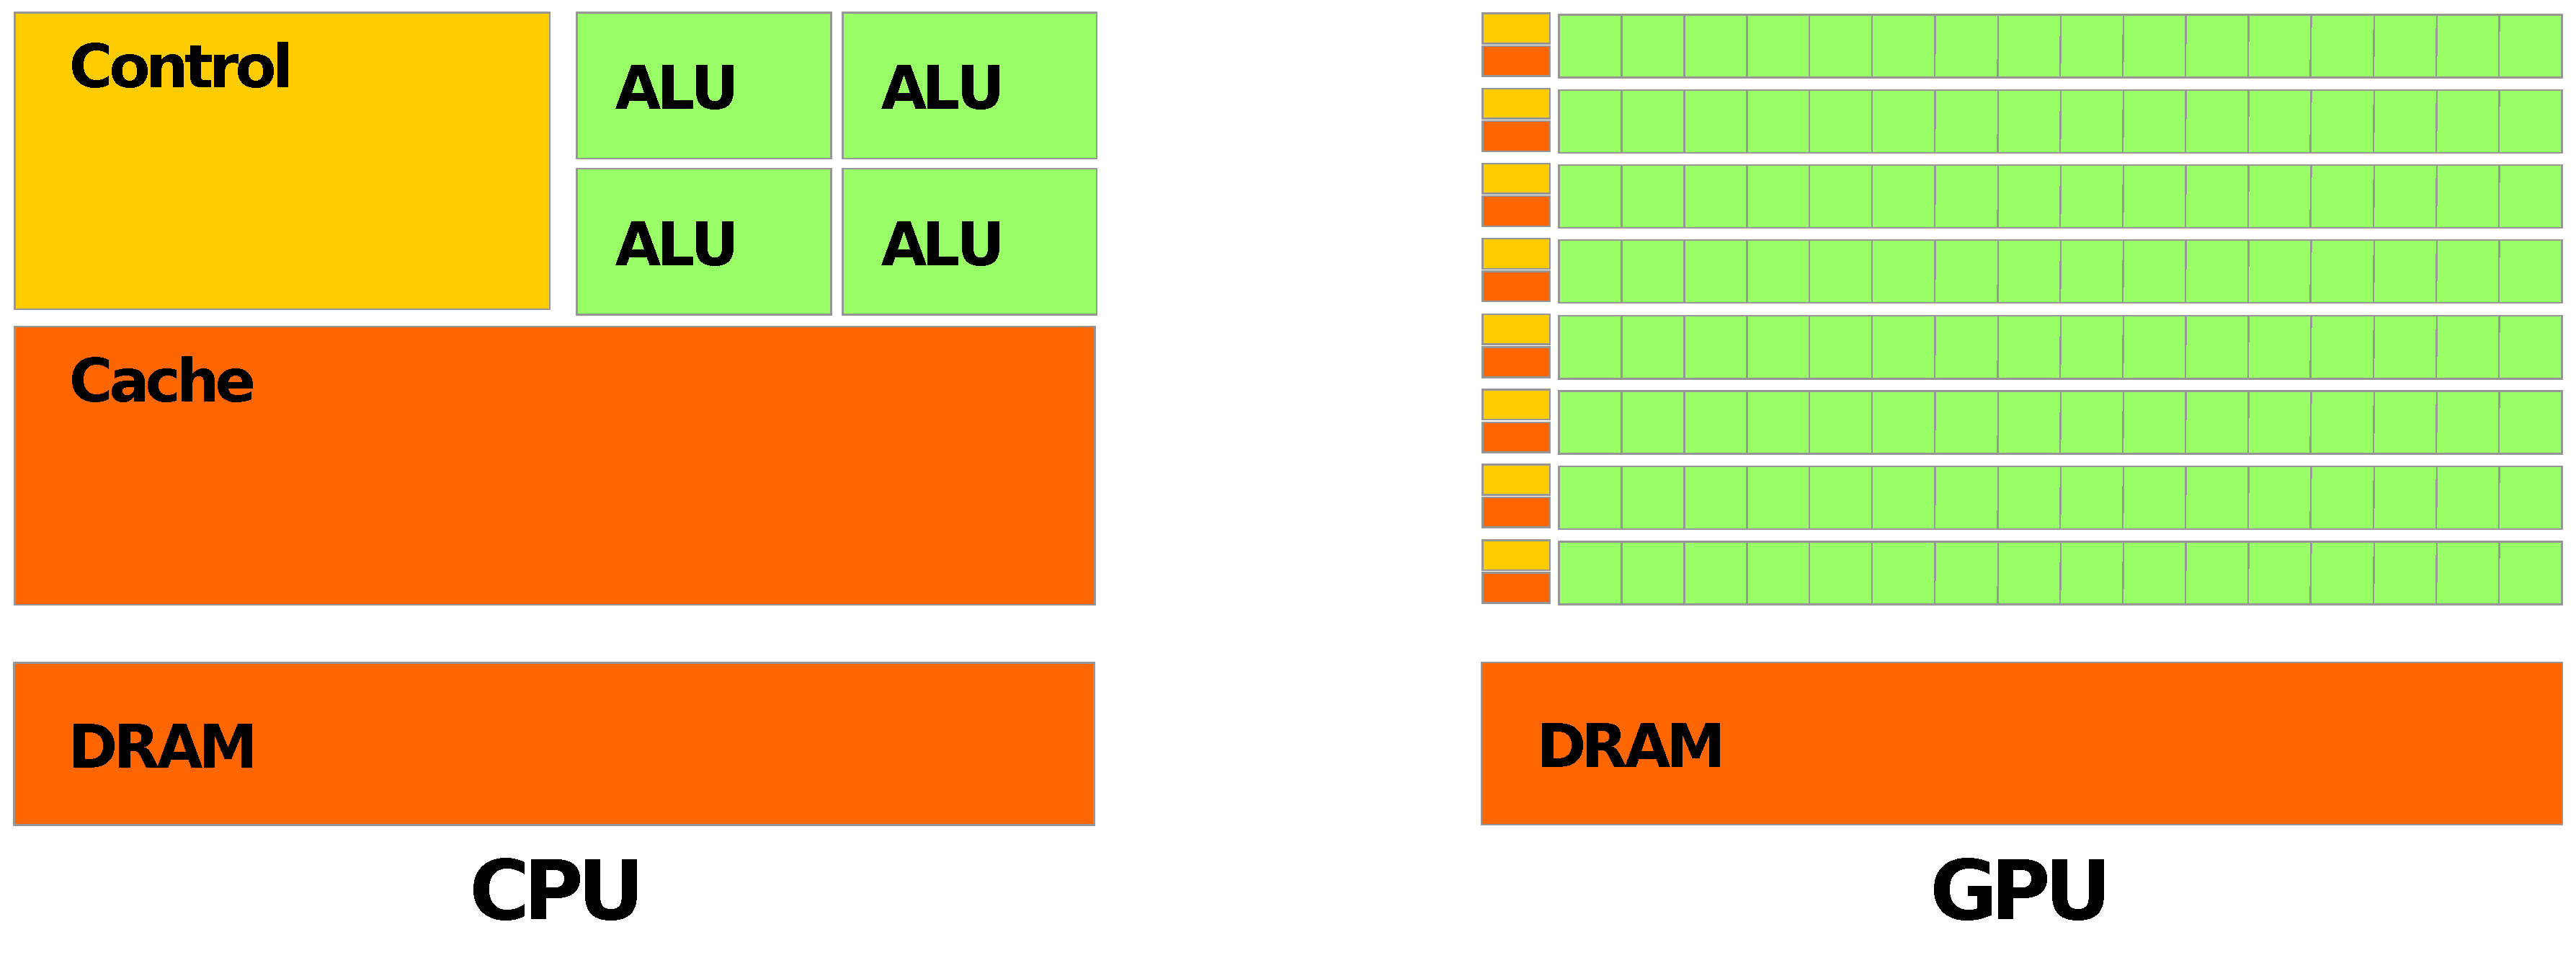
\includegraphics[width=\linewidth]{images/gpu-vs-cpu.eps}
        \caption{CPU vs GPU architecture\protect\footnotemark}
      \end{figure}
      
      \footnotetext{Copyright \textcopyright~2010, NVIDIA Corporation, published under a \href{https://creativecommons.org/licenses/by/3.0/}{Creative Commons Attribution 3.0 Unported License}; source: \url{https://commons.wikimedia.org/w/index.php?title=File:Cpu-gpu.svg&oldid=156649300}}
      
      Streaming multiprocessors are designed for \emph{data parallelism} -- each thread should ideally execute the same sequence of instructions over different data. The workload given to a GPU consists of a certain number of executions (\emph{threads}) of a single program (\emph{kernel}). Threads are divided into \emph{blocks}, which are distributed among SMs. Blocks are further divided into smaller \emph{warps} of threads -- all threads in a warp always execute the same instruction. SM can switch between currently running warps, for example to hide memory latency while a warp waits for a memory transaction. Warp scheduling is handled by hardware automatically, which minimizes scheduling overhead \cite{nvidia:gpuArch}.
      
      Kernels may contain branches and loops -- in this case, both paths of each branch are executed in each thread. Branching should, however, be used carefully -- if the threads within a warp diverge (that is, they end up executing different parts of the kernel) the computation becomes inefficient. As opposed to CPUs, SMs in GPUs always execute instructions in-order instead of out-of-order. Memory latency is avoided by temporarily switching to another warp \cite{nvidia:gpuArch}.
            
      Each streaming multiprocessor contains a single \emph{instruction unit} (similar to the CPU's control unit) with instruction cache, \emph{constant cache} (a cache for the part of global memory which contains constant data), \emph{shared memory}, several \emph{thread processors} (denoted SP) and several \emph{special function units} (SFU) \cite{nvidia:gpuArch}. SPs execute arithmetic instructions, SFUs are used for special mathematical functions, such as sine, cosine or logarithm \cite{nvidia:gpuArch}.
      
      \begin{figure}
        \centering
        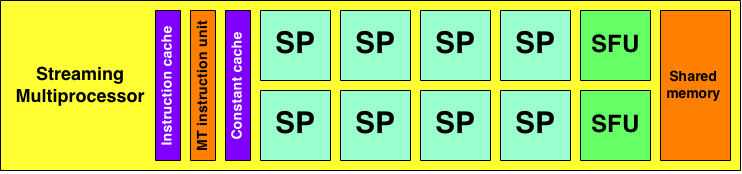
\includegraphics[width=\linewidth]{images/sm.png}
        \caption{Streaming multiprocessor\protect\footnotemark}
      \end{figure}
      \footnotetext{The picture was adapted from \cite{nvidia:gpuArch}.}
      
      \section{Memory hierarchy}
      \begin{figure}
        \centering
        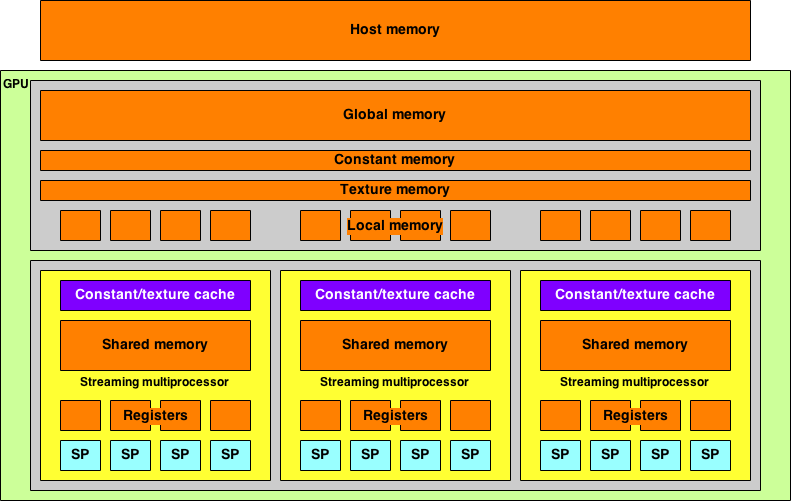
\includegraphics[width=\linewidth]{images/gpu-memory.png}
        \caption{GPU memory hierarchy}
      \end{figure}
      
      \subsection{Global memory}
      The main memory of a GPU is the \emph{global memory}. Global memory is a dynamic random-access memory (DRAM), which is the type of memory that is also typically used for a computer's main memory. Accessing global memory from a thread has a relatively high latency (as opposed to registers), because it is not cached (except for the part that is reserved for constant data). The size of global memory ranges from hundreds  of megabytes to several gigabytes \cite{wiki:listOfGPUs}.
      
      \subsection{Constant memory}
      Part of global memory is used as the so-called \emph{constant memory}. To the threads running on the GPU the constant memory is read-only. Since constant memory is cached, accessing it from a thread has relatively low latency (unless there is a cache miss, it can be as fast as the registers). Usage of constant memory is optimal when all threads in a warp are reading the same memory location at once \cite[section 5.3.2., Constant memory]{nvidia:cudaProgGuide}. The size of constant memory in CUDA is fixed to 64 KB with 8-10 KB of cache for each streaming multiprocessor \cite[appendix G.1]{nvidia:cudaProgGuide}.
      
      \subsection{Texture memory}
      Another part of global memory is used as \emph{texture memory}. Like constant memory, texture memory is also cached. Texture memory is, as opposed to constant memory, optimized for two-dimensional spacial locality. That is, the data in the memory is interpreted as a two-dimensional array of values and accesses to the memory are optimal when threads in the same warp access memory locations that correspond to positions in the array that are close to each other \cite[section 5.3.2., Texture memory]{nvidia:cudaProgGuide}.
      
      \subsection{Local memory}
      The GPU driver also allocates a block of global memory as the \emph{local memory} for each thread (if necessary). Local memory is used for thread-local data that does not fit into the registers in the streaming multiprocessor \cite[section 5.3.2., Local memory]{nvidia:cudaProgGuide}. Since accesses to the local memory have a high latency, the programmer should keep the per-thread data as small as possible, so that only SM registers are used.
      
      \subsection{Shared memory}
      Each streaming multiprocessor contains an on-chip \emph{shared memory} which is shared between threads in the same block. The shared memory is distributed among blocks that are being executed by the SM. The size of the shared memory is typically about 16 KB. Shared memory has higher throughput and lower latency than global memory \cite[section 5.3.2., Shared memory]{nvidia:cudaProgGuide}.
      
      Shared memory is divided into modules of the same size called \emph{banks}. When threads each access a different bank, the data transfer can be performed in parallel. When two or more threads access the same bank, the access has to be serialized \cite[section 5.3.2., Shared memory]{nvidia:cudaProgGuide}.
      
      \subsection{Registers}
      The fastest kind of memory available on a GPU are the registers within SPs. The registers are divided among all threads in a block -- the registers for each block remain allocated until all threads in the block finish execution, which allows for fast warp switching.
      
    \chapter{Implementing a brute-force attack on PBKDF2 on GPUs}
      In this chapter we discuss the feasibility of an efficient brute-force attack on the PBKDF2 key derivation function. We focus on the PBKDF2-HMAC family of functions\footnote{by PBKDF2-HMAC we denote the family of functions that use HMAC-\emph{hash} (for any \emph{hash}) as their underlying PRF} as these are most frequently used in real-world applications (see section \ref{s:PBKDF2}).
      
      \section{Notes on implementing PBKDF2-HMAC}
      Let $H$ be a hash function that uses an internal state of $s$ octets, operates on input blocks of $b$ octets and produces output of $l$ octets ($l \le s$, $l \le b$). We shall assume that the hash function is defined by the following parameters:
      \begin{itemize}
        \item $H_I$ -- the initial state (an octet string of length $s$),
        \item $H_U$ -- the \emph{update} function, which takes the previous state (an octet string of length $s$) and an input block (an octet string of length $b$) and returns the new state (an octet string of length $s$),
        \item $H_F$ -- the \emph{finalize} function, which takes the previous state (an octet string of length $s$), the last (possibly incomplete) input block (an octet string of length at most $b$) and the total length of the input string (a non-negative integer) and returns the final hash (an octet string of length $l$).
      \end{itemize}
      We further assume that computing the hash function $H$ over an input octet string $D$ of length $n$ proceeds as follows:
      \begin{algorithmic}[1]
        \Function{$H$}{$D$, $n$}
          \State $S \gets H_I$
          \State $c \gets \lceil n / b \rceil - 1$
          \For{$i \gets 1$, $c$}
            \State $S \gets H_U(S, D[ib:(i+1)b-1])$
          \EndFor
          \State \Return $H_F(S, D[cb:n-1], n)$
        \EndFunction
      \end{algorithmic}
      
      Here, $A[i..k]$ denotes an octet string produced by taking the $i$-th through the $k$-th octet of the octet string $A$.
      
      It can be shown that any hash function that uses the Merkle-Damgård construction (see \cite[p. 333]{handbook}; this includes all of the commonly used hash functions -- SHA-1, SHA-2, SHA-3, MD4, MD5, RIPEMD, Whirlpool) conforms to this definition.
      
      \paragraph*{}
      Following the above definition and the HMAC specification (\cite{rfc2104}) the pseudocode from section \ref{s:PBKDF2} can be rewritten for PBKDF2-HMAC as follows:
      \begin{algorithmic}[1]
        \Function{PBKDF2-HMAC}{$P, S, c, dkLen$}
          \If{$dkLen \le (2^{32} - 1) \cdot hLen$}
            \State output ``derived key too long'' and stop
          \EndIf
          \State $l \gets \lceil dkLen / hLen\rceil$ \Comment{{\footnotesize $l$ is the number of $hLen$-octet blocks in the derived key, rounding up}}
          \State $r \gets dkLen - (l - 1) \cdot hLen$ \Comment{{\footnotesize $r$ is the number of octets in the last block}}
          \State \Comment{{\footnotesize Pre-hash the password if necessary and pad it with zeroes:}}
          \If{$|P| > b$}
            \State $K \gets H(P)|\operatorname{repeat}(\text{0x00}, b - l)$
          \Else
            \State $K \gets P|\operatorname{repeat}(\text{0x00}, b - |P|)$
          \EndIf
          \State \Comment{{\footnotesize Setup \emph{ipad} and \emph{opad} partial hash states:}}
          \State $S_{IPAD} \gets H_U(H_I, K \oplus \operatorname{repeat}(\text{0x36}, b))$
          \State $S_{OPAD} \gets H_U(H_I, K \oplus \operatorname{repeat}(\text{0x5C}, b))$
          \For{$k \gets 1$, $l$} \label{dkLoop:from}
            \State \Comment{{\footnotesize The first iteration:}}
            \State $A \gets S \mid \operatorname{int}(k)$
            \State $c_A \gets \lfloor |A| / b \rfloor$
            \State $S_{SALT} \gets S_{IPAD}$
            \For{$i \gets 1$, $c_A$}
              \State $S_{SALT} \gets H_U(S_{SALT}, A[ib:(i+1)b-1])$
            \EndFor
            \State $T_k \gets H_F(S_{OPAD}, H_F(S_{SALT}, A[c_Ab:|A|-1]))$
            \State \Comment{{\footnotesize The remaining iterations:}}
            \For{$i \gets 2$, $c$} \label{mainLoop:from}
              \State $D \gets H_F(S_{IPAD}, T_k)$
              \State $D \gets H_F(S_{OPAD}, D)$
              \State $T_k \gets T_k \oplus D$
            \EndFor \label{mainLoop:to}
          \EndFor \label{dkLoop:to}
          \State \Return $T_1 \mid T_2 \mid ... \mid T_l[0..r - 1]$
        \EndFunction
      \end{algorithmic}
      
      Here, $|A|$ denotes the length of octet string $A$; $\operatorname{repeat}(x, n)$ denotes an octet string produced by repeating octet $x$ $n$ times; 0x$XY$ denotes an octet in hexadecimal representation.
      
      \paragraph*{}
      When trying to implement PBKDF2 efficiently, the most important part for optimization is the main loop from lines \ref{mainLoop:from}-\ref{mainLoop:to}, as this is the only part, time complexity of which depends on the number of iterations. When HMAC is used as the PRF in PBKDF2, this part is very simple -- it iteratively performs two hashing operations over the result of the previous iteration and then combines the result with the result of the previous iteration. Therefore, assuming a reasonably high iteration count, in order to optimize PBKDF2-HMAC it is sufficient to optimize the implementation of the underlying hash function.
      
      On parallel computing platforms such as GPUs, it is also important that the computation consumes as little memory as possible. When PBKDF2 is used with HMAC as the PRF, the memory requirements of the core of the algorithm (the main loop from the previous paragraph) do not depend on the security parameters (iteration count, salt length), but only depend on the hash function used. For example, with SHA-1 used as the hash, the core of the algorithm requires approximately 164 bytes (plus few more bytes might be required for temporary variables); with SHA-256 it requires approximately 224 bytes and with SHA-512 approximately 448 bytes.
      
      \section{Running PBKDF2 on a GPU} \label{s:PBKDF2onGPU}
      PBKDF2-HMAC, when used with common hash functions, has several properties that make it possible to implement it very efficiently on GPU hardware (for bulk processing). This poses a security/usability problem for applications that cannot utilize the GPU for evaluating PBKDF2 (this is true for almost all practical applications, with only a few exceptions -- e. g. busy user authentication servers). The great difference in performance between the hardware available to the user and the hardware available to the attacker means that in order to provide reasonable security, the PBKDF2 iteration count must be set according to the attacker's potential hardware capabilities, which in turn causes an excessive inconvenience to the user, who then has to wait a long time for the password to be processed.
      
      \paragraph*{}
      As with most cryptographic algorithms, an efficient implementation PBKDF-HMAC does not require any data-dependent branching (executing different code on different inputs) which avoids divergence of different GPU threads (see chapter \ref{ch:gpuArch}). This is, however, a desirable security property that helps prevent timing attacks, where an attacker attempts to gain information about a secret parameter by measuring and analyzing the time it takes to perform a certain cryptographic function.
      
      Another important property of PBKDF2-HMAC is that it has constant and very low memory requirements (as discussed in the previous section). This allows the GPU implementation to run more threads while keeping most (or all) of the data in the registers, thus avoiding expensive accesses to the global memory. As discussed on page \pageref{p:memoryHard}, new password-based key derivation functions (such as scrypt) address this problem by using so called \emph{sequential memory-hard functions}.
      
      An interesting property of PBKDF2-HMAC is also the fact that each hash-output-sized block of the derived key can be computed independently. This allows the GPU implementation to compute each block in a separate thread, which means that when deriving longer keys, fewer PBKDF2 tasks are sufficient to saturate all cores of the GPU. This, however, does not provide a significant advantage for brute-force/dictionary attacks, as the attacker has a lot of tasks to process and can always submit more of them at once.
      
    \chapter{The demonstration program}
      To demonstrate how GPUs can be used to accelerate a brute-force or dictionary attack on a real-world system that uses PBKDF2 for password-based key derivation, we implemented a simple demonstration program in the form of a command-line application that performs an offline attack on the access passwords of a LUKS partition.
      
      The source code of the demonstration program can be found in the source code archive included in the thesis repository, under the \texttt{lukscrack-gpu} directory. The source code is also accessible online as a GitHub repository\footnote{\url{https://github.com/WOnder93/pbkdf2-gpu}}. Appendix \ref{a:docs} contains the documentation for building and running this program.
      
      \section{An introduction to LUKS} \label{s:luks}
      LUKS (Linux Unified Key Setup) is a standard for key setup\footnote{key setup = the management of encryption keys used in a cryptosystem} in disk encryption \cite{luks}. It was originally developed for the purpose of standardizing and simplifying the process of key management for disk encryption on the Linux operating system \cite[chapter 6]{Fruhwirth}. Nevertheless, the standard itself is platform independent and can be implemented on any platform.
      
      LUKS defines a binary format for storing keys and encrypted data on disk partitions, as well as basic operations on partitions which use this format (partition initialization, adding, changing and revoking passwords, etc.) \cite{luks}. In this section we describe LUKS version 1.2.1, which is the latest version to date (14 May 2015).
      
      \paragraph*{}
      A LUKS partition begins with a \emph{partition header}, followed by eight sections of encrypted key data (called \emph{key material}), which is then followed by the encrypted \emph{payload} (the data stored on the partition).
      
      The payload of a LUKS partition is encrypted by a \emph{master key}\footnote{The term \emph{master key} is used by the LUKS specification. In other literature the key used to encrypt partition data is usually called the \emph{volume key}.} (MK), which is randomly generated when initializing the partition and does not change during the lifetime of the partition.
      
      The partition header contains information about eight \emph{key slots}, each of which can be active or disabled. Each active key slot is associated with one of the key material sections. Each key material section contains the master key processed by a transformation called \emph{AFsplit}\footnote{\emph{AF} stands for anti-forensic.} (explained below) and encrypted with a key derived from the \emph{user password}. Each key slot contains parameters that specify how to obtain the master key from the associated key material and the corresponding user password. This means that the user needs to know the correct password of at least one key slot in order to decrypt the whole partition.
      
      A more detailed description of the LUKS partition format can be found in the LUKS On-Disk Format Specification \cite[section 2.4]{luks}.
      
      \subsection{AFsplit}
      The master key is usually only 16 or 32 bytes long \cite[chapter 1]{luks}. Therefore when stored on a hard disk device, it is likely to end up in a single physical disk sector. When a disk sector gets damaged or corrupted, the disk firmware may silently remap it another spare sector and the original sector becomes inaccessible \cite[chapter 1]{luks}. Even though the remapped sector becomes inaccessible to the software and is likely unreadable, an advanced forensic analysis might still be able to recover all or part of the data stored in the sector.
      
      Suppose an encrypted master key was stored in a single sector, which was later remapped to another sector. If the key used to encrypt the MK was then revoked, the disk encryption software, not knowing that the remapping occurred, would only erase the new sector, while the data might still be readable from the original one.
      
      To counter this problem, LUKS defines a transformation called \emph{AFsplit} (the inverse transformation is called \emph{AFmerge}), which transforms a key (any octet string) into an octet string, size of which is an arbitrary multiple of the key size and such that the master key can only be recovered from the whole string.
      
      In theory, the whole key material section could be remapped before it is erased (when the key is revoked). Therefore, in order to completely prevent key recovery from remapped sectors, the size of the key material must be greater than the total size of the spare sectors available on the disk device. On solid-state disk drives the total size of spare disk sectors often exceeds the practical size of the key material, thus this countermeasure may not provide sufficient security on these devices.
      
      A brief definition of the AFsplit/AFmerge transformation can be found in \cite[section 2.4]{luks}. A more detailed description and rationale is provided by Fruhwirth in \cite[section 5.2]{Fruhwirth}.
      
      \subsection{Verifying LUKS partition passwords}
      To implement a brute-force attack on a LUKS partition, it is essential to understand the process of verifying whether a password is valid for a given active key slot. In order to verify a key slot password, the following fields of the partition header are needed (field names are as per \cite{luks}):
      \begin{itemize}
        \item \emph{cipher-name}, \emph{cipher-mode} -- text identifiers of the cipher (encryption algorithm) that is used to encrypt the key material (and to encrypt the payload),
        \item \emph{hash-spec} -- a text identifier of the hash function used for key derivation, the AFsplit/AFmerge transformation and for computing the master key digest (see below),
        \item \emph{key-bytes} -- the length in bytes of the key used with the cipher specified by \emph{cipher-name} and \emph{cipher-mode} (that is, the master key and the key material encryption key),
        \item \emph{mk-digest} -- the master key digest, which is computed from the MK using PBKDF2-HMAC with the hash function specified by \emph{hash-spec},
        \item \emph{mk-digest-salt}, \emph{mk-digest-iter} -- the PBKDF2 salt and iteration count used for computing the MK digest.
      \end{itemize}
      
      In addition to this information, the following fields of the key slot are needed:
      \begin{itemize}
        \item \emph{iterations}, \emph{salt} -- the PBKDF2 iteration count and salt used for deriving the key material encryption key from the user password,
        \item \emph{key-material-offset} -- the offset in sectors\footnote{a sector in LUKS is 512 bytes long (this fact is omitted in version 1.2.1 of the LUKS On-Disk Format Specification)} of the key material associated with the key slot,
        \item \emph{stripes} -- the factor by which the MK is expanded by the AFsplit transformation.
      \end{itemize}
      
      \begin{figure}[t]
        \centering
        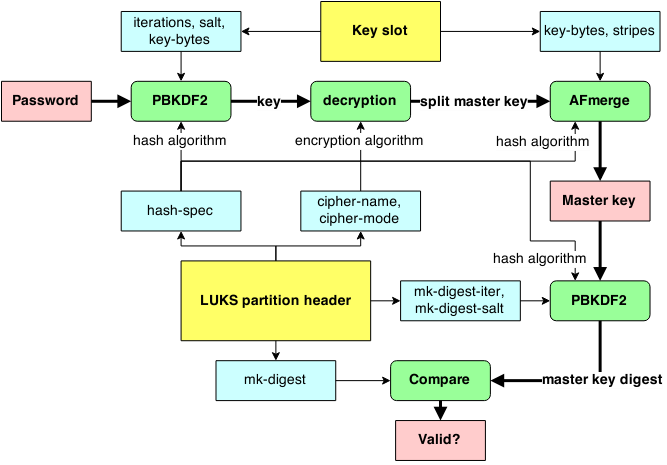
\includegraphics[width=\linewidth]{images/luks-pwcheck.png}
        \caption{LUKS partition password verification}
      \end{figure}
      
      Using the information above, the key slot password verification proceeds as follows:
      \begin{enumerate}
        \item The key material sectors are read from the partition. The key material starts at sector specified by \emph{key-material-offset} and takes up as many sectors as needed to store \emph{key-bytes} times \emph{stripes} bytes.
        \item A key of \emph{key-bytes} bytes is derived from the password using PBKDF2-HMAC with the hash function specified by \emph{hash-spec}, the value of the \emph{iterations} field as the iteration count and the contents of the \emph{salt} field as the salt.
        \item The derived key from the previous step is used to decrypt the key material sectors. The first \emph{key-bytes} times \emph{stripes} bytes of the decrypted data are taken as the split master key. The trailing bytes (if any) are ignored.
        \item The master key candidate is obtained from the split master key by applying the AFmerge transformation with the hash function specified by \emph{hash-spec}, with \emph{key-bytes} as the key length and with \emph{stripes} as the expansion factor.
        \item Finally, a 20-byte digest\footnote{This is a relic from when LUKS only supported SHA-1 as the hash function (the output of SHA-1 is 20 bytes long).} of the master key candidate is produced by applying PBKDF2-HMAC with the hash function specified by \emph{hash-spec}, \emph{mk-digest-iter} as the iteration count and \emph{mk-digest-salt} as the salt. The computed digest is then compared to \emph{mk-digest} -- if the digests match, the password is valid, otherwise it is not.
      \end{enumerate}
      
      \section{Implementation} \label{s:demoProgImpl}
      As shown in the previous section, verifying a LUKS key slot password requires two computations of PBKDF2, between which a different computation needs to be performed (key material decryption and AFmerge).
      
      For a typical LUKS partition created by cryptsetup the most computationally difficult is the first PBKDF2 instance (deriving encryption key from the password). The second PBKDF2 instance (master key digest computation) is about 8 times less computationally difficult and the difficulty of the rest of the computation is usually negligible. In our demonstration program both PBKDF2 instances are computed on the GPU, while the rest of the computation is performed on the CPU.
      
      \subsection{Optimal utilization of hardware resources}
      In order to employ all cores of the GPU, our demonstration program processes the candidate passwords in \emph{batches}. The state of processing a password batch is managed by an object which we call the \emph{batch processing context} (BPC). The BPC can be thought of as a state machine with four states (excluding the initial and final state) where the transitions between states represent separate stages of computation. Figure \ref{fig:processingContext} shows a state diagram of the BPC.
      
      \begin{figure}[t]
        \centering
        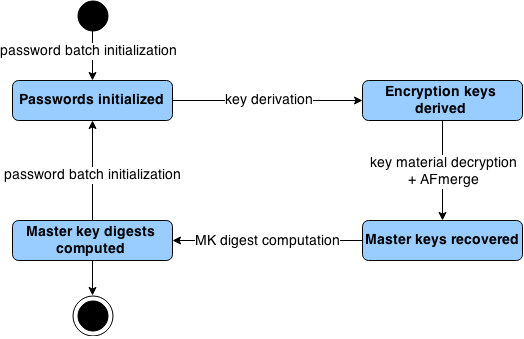
\includegraphics[width=\linewidth]{images/bpc.png}
        \caption{Batch processing context -- a state diagram}
        \label{fig:processingContext}
      \end{figure}
      
      %TODO ?describe also in text
      
      \paragraph*{}
      Since most of the computation is performed on the GPU, it is desirable that it is kept fully utilized throughout the attack. Also, in case the GPU used was so powerful that the CPU computation takes longer than the GPU computation, it would be preferable if the CPU was kept fully utilized.
      
      For this reason, we devised a simple scheduling algorithm which coordinates execution of three concurrent BPCs in a way that ensures that the computing hardware is optimally utilized (as described in the previous paragraph).
      
      \begin{algorithm}
        \caption{Batch processing context scheduling}
        \label{alg:bpcSched}
        \begin{algorithmic}[1]
          \Procedure{CpuPhase1}{bpc}
            \State \Call{EndMkDigestComputation}{bpc}
            \State \Call{ProcessDigests}{bpc}
            \State \Call{InitPasswords}{bpc}
            \State \Call{BeginKeyDerivation}{bpc}
          \EndProcedure
          \State
          \Procedure{CpuPhase2}{bpc}
            \State \Call{EndKeyDerivation}{bpc}
            \State \Call{DecryptKeyMaterial}{bpc}
            \State \Call{BeginMkDigestComputation}{bpc}
          \EndProcedure
          \State
          \Procedure{ProcessPasswords}{bpc1, bpc2, bpc3}
            \State (run a partial version of the body of the loop below to initialize the BPCs to the loop's invariant)
            \While{(there are passwords to process)}
              \State \Call{CpuPhase1}{bpc1}
              \State \Call{CpuPhase2}{bpc3}
              \State \Call{CpuPhase1}{bpc2}
              \State \Call{CpuPhase2}{bpc1}
              \State \Call{CpuPhase1}{bpc3}
              \State \Call{CpuPhase2}{bpc2}
            \EndWhile
            \State (run a partial version of the body of the loop above to finalize the BPCs from the loop's invariant)
          \EndProcedure
        \end{algorithmic}
      \end{algorithm}
      
      The algorithm is informally described in the pseudocode of the \Call{ProcessPasswords}{} procedure presented in algorithm \ref{alg:bpcSched}. An explanation of the procedures used in algorithm \ref{alg:bpcSched} follows:
      \begin{itemize}
        \item \Call{InitPasswords}{\emph{bpc}} -- initializes \emph{bpc} with a new password batch.
        \item \Call{BeginKeyDerivation}{\emph{bpc}} -- submits the PBKDF2 task to derive the keys for key material decryption from the passwords to the GPU.
        \item \Call{EndKeyDerivation}{\emph{bpc}} -- waits for the task submitted by \Call{BeginKeyDerivation}{\emph{bpc}} to end.
        \item \Call{DecryptKeyMaterial}{\emph{bpc}} -- decrypts the key material using the derived keys, then obtains MK candidates from the decrypted versions of the key material using the AFmerge transformation.
        \item \Call{BeginMkDigestComputation}{\emph{bpc}} -- submits the PBKDF2 task to compute digests of the MK candidates to the GPU (for the BPC \emph{bpc}).
        \item \Call{EndMkDigestComputation}{\emph{bpc}} -- waits for the task submitted by \Call{BeginMkDigestComputation}{\emph{bpc}} to end.
        \item \Call{ProcessDigests}{\emph{bpc}} -- compares the computed MK candidate digests with the MK digest from the partition header. If a matching digest is found, reports that a valid password was found and stops the processing.
      \end{itemize}
      
      The GPU tasks are executed one at a time in the order in which they have been submitted.
      
      \begin{figure}
        \centering
        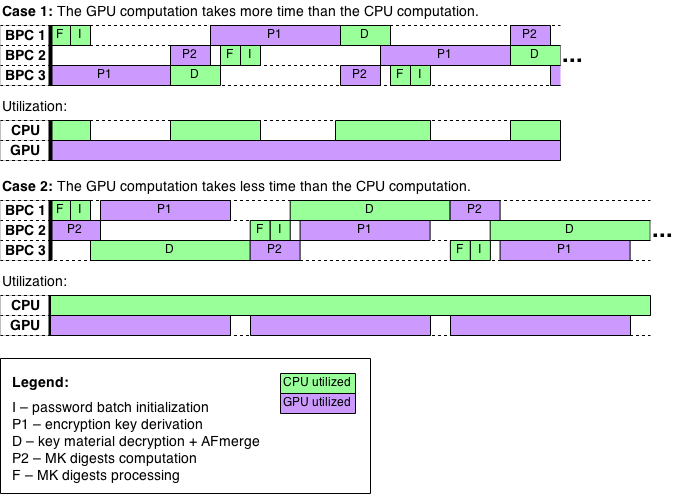
\includegraphics[width=\linewidth]{images/scheduling.png}
        \caption{The scheduling algorithm -- resource utilization}
        \label{fig:scheduling}
      \end{figure}
      
      Figure \ref{fig:scheduling} shows how our algorithm achieves optimal CPU/GPU utilization in both cases discussed earlier in this section.
      
      \subsection{Using multiple CPU threads or GPUs}
      The demonstration program allows the user to specify multiple GPUs to use for computation of PBKDF2, as well as the number of CPU threads to use for the key material decryption and AFmerge transformation phase.
      
      \paragraph*{}
      When the user specifies multiple GPUs to be used, the program runs processing on each GPU separately. That is, each GPU is controlled from a separate CPU thread, which executes a separate set of interleaved batch processing contexts as described in the previous subsection.
      
      \paragraph*{}
      When the user specifies that more than one CPU thread should be used, the program allocates the requested number of threads which share a synchronized queue from which they pull the tasks to execute. All GPU controlling threads have a reference to the queue and push tasks into it. When a GPU controlling thread needs to perform key material decryption and AFmerge transformation over a batch of inputs, the inputs are divided into as many groups of approximately equal size as there are CPU threads allocated. For each group a separate task that processes the inputs in the group is pushed to the queue. The GPU controlling thread then waits for all tasks it has pushed to the queue to complete.
      
      Figure \ref{fig:lukscrackArch} shows an illustration of the overall architecture as described in this subsection.
      
      \begin{figure}
        \centering
        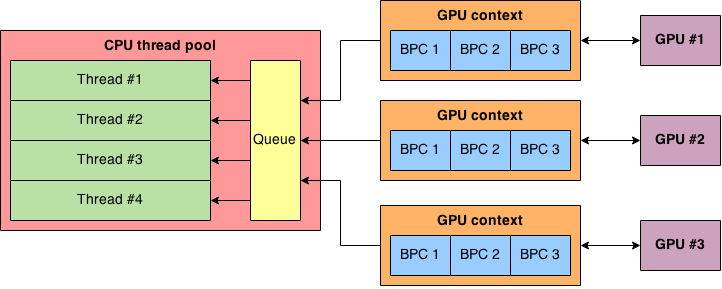
\includegraphics[width=\linewidth]{images/lukscrack-gpu-architecture.png}
        \caption{The overall architecture of the demonstration program}
        \label{fig:lukscrackArch}
      \end{figure}
      
      \paragraph*{}
      If the user specifies that only one CPU thread should be used, then no extra threads are allocated and all CPU computation is performed directly in each GPU controlling thread.
      
    \chapter{Comparison of CPU and GPU attack speeds}
      In order to compare the potential speed of a brute-force/dictionary attack on the PBKDF2 key derivation function, we wrote a GPU implementation of PBKDF2-HMAC-SHA1 and ran benchmarks on both the GPU implementation and a CPU reference implementation on various devices.
      
      The source code of the benchmarking program as well as the raw measurement data can be found in the source code archive included in the thesis repository, under the \texttt{benchmarking-tool} directory. The source code is also accessible online as a GitHub repository\footnote{\url{https://github.com/WOnder93/pbkdf2-gpu}}. Appendix \ref{a:docs} contains the documentation for building and running the benchmarking program.
      
      \section{Implementation and methodology}
      In the GPU implementation, we used the OpenCL API for submitting work to the GPU.
      
      In order to utilize all cores of the GPU and therefore maximize the performance, our implementation processes passwords in large fixed-size batches. The optimal password batch size varies between devices and can be specified by the user.
      
      The implementation works as follows:
      \begin{enumerate}
        \item A new password batch is initialized on the host CPU (in the benchmarking program the passwords are initialized to fixed-length pseudorandom strings). Each password is pre-hashed and padded with zeroes if necessary as per the HMAC specification \cite{rfc2104}. The resulting fixed-size blocks are transferred to the global memory on the GPU.
        
              The initialization and memory transfer are not included in the benchmark, since in a practical attack they can be performed while the GPU is processing another password batch, and thus have no effect on the attack speed.
        \item Next, the work is submitted to the GPU. One GPU thread is assigned for each hash-output-sized block of the derived key of each password (see section \ref{s:PBKDF2onGPU}).
        \item The CPU thread waits for the GPU to finish processing the password batch and the difference between the time the work was submitted and the time the waiting finished is taken as the result of the benchmark.
      \end{enumerate}
      
      The CPU implementation uses the API of the OpenSSL \emph{crypto} library\footnote{\url{https://www.openssl.org/docs/}}, specifically the PKCS5\_PBKDF2\_HMAC function. The benchmarks were run with the LibreSSL library\footnote{\url{https://github.com/libressl-portable/portable}} due to problems when building the OpenSSL library on the system where the benchmarks were run.
      
      All benchmarks were run on machines provided by MetaCentrum\footnote{\url{https://metavo.metacentrum.cz/en/index.html}} running the Linux operating system.
      
      Due to the variance in running times, the benchmarks were run several times for each data point and the arithmetic mean was taken as the final value. For GPU benchmarks the number of samples was 10, for CPU benchmarks it was 20 (the variance in running times for the GPU implementation was smaller than for the CPU implementation).
      
      \section{Results} \label{s:results}
      The results of the benchmarks show that a brute-force attack on PBKDF2-HMAC-SHA1 can be performed very efficiently on GPU hardware. The GPU implementation significantly outperforms the reference CPU implementation both in terms of attack speed per single device and in terms of power efficiency.
      
      Figure \ref{graph:devices:speed} shows a comparison of attack speeds for various devices. The attack speed is measured in PBKDF2 block-iterations per second (PBIPS) -- that is the number of PBKDF2 instances (i. e. the number of passwords processed) times the number of blocks of the derived key computed independently times the iteration count over the time it took to process these passwords. We use this unit because the amount of computation needed to perform one PBKDF2 instance is proportional to the iteration count and to the smallest number of hash-output-sized blocks such that they can fit the derived key.
      
      \begin{figure}
        \centering
        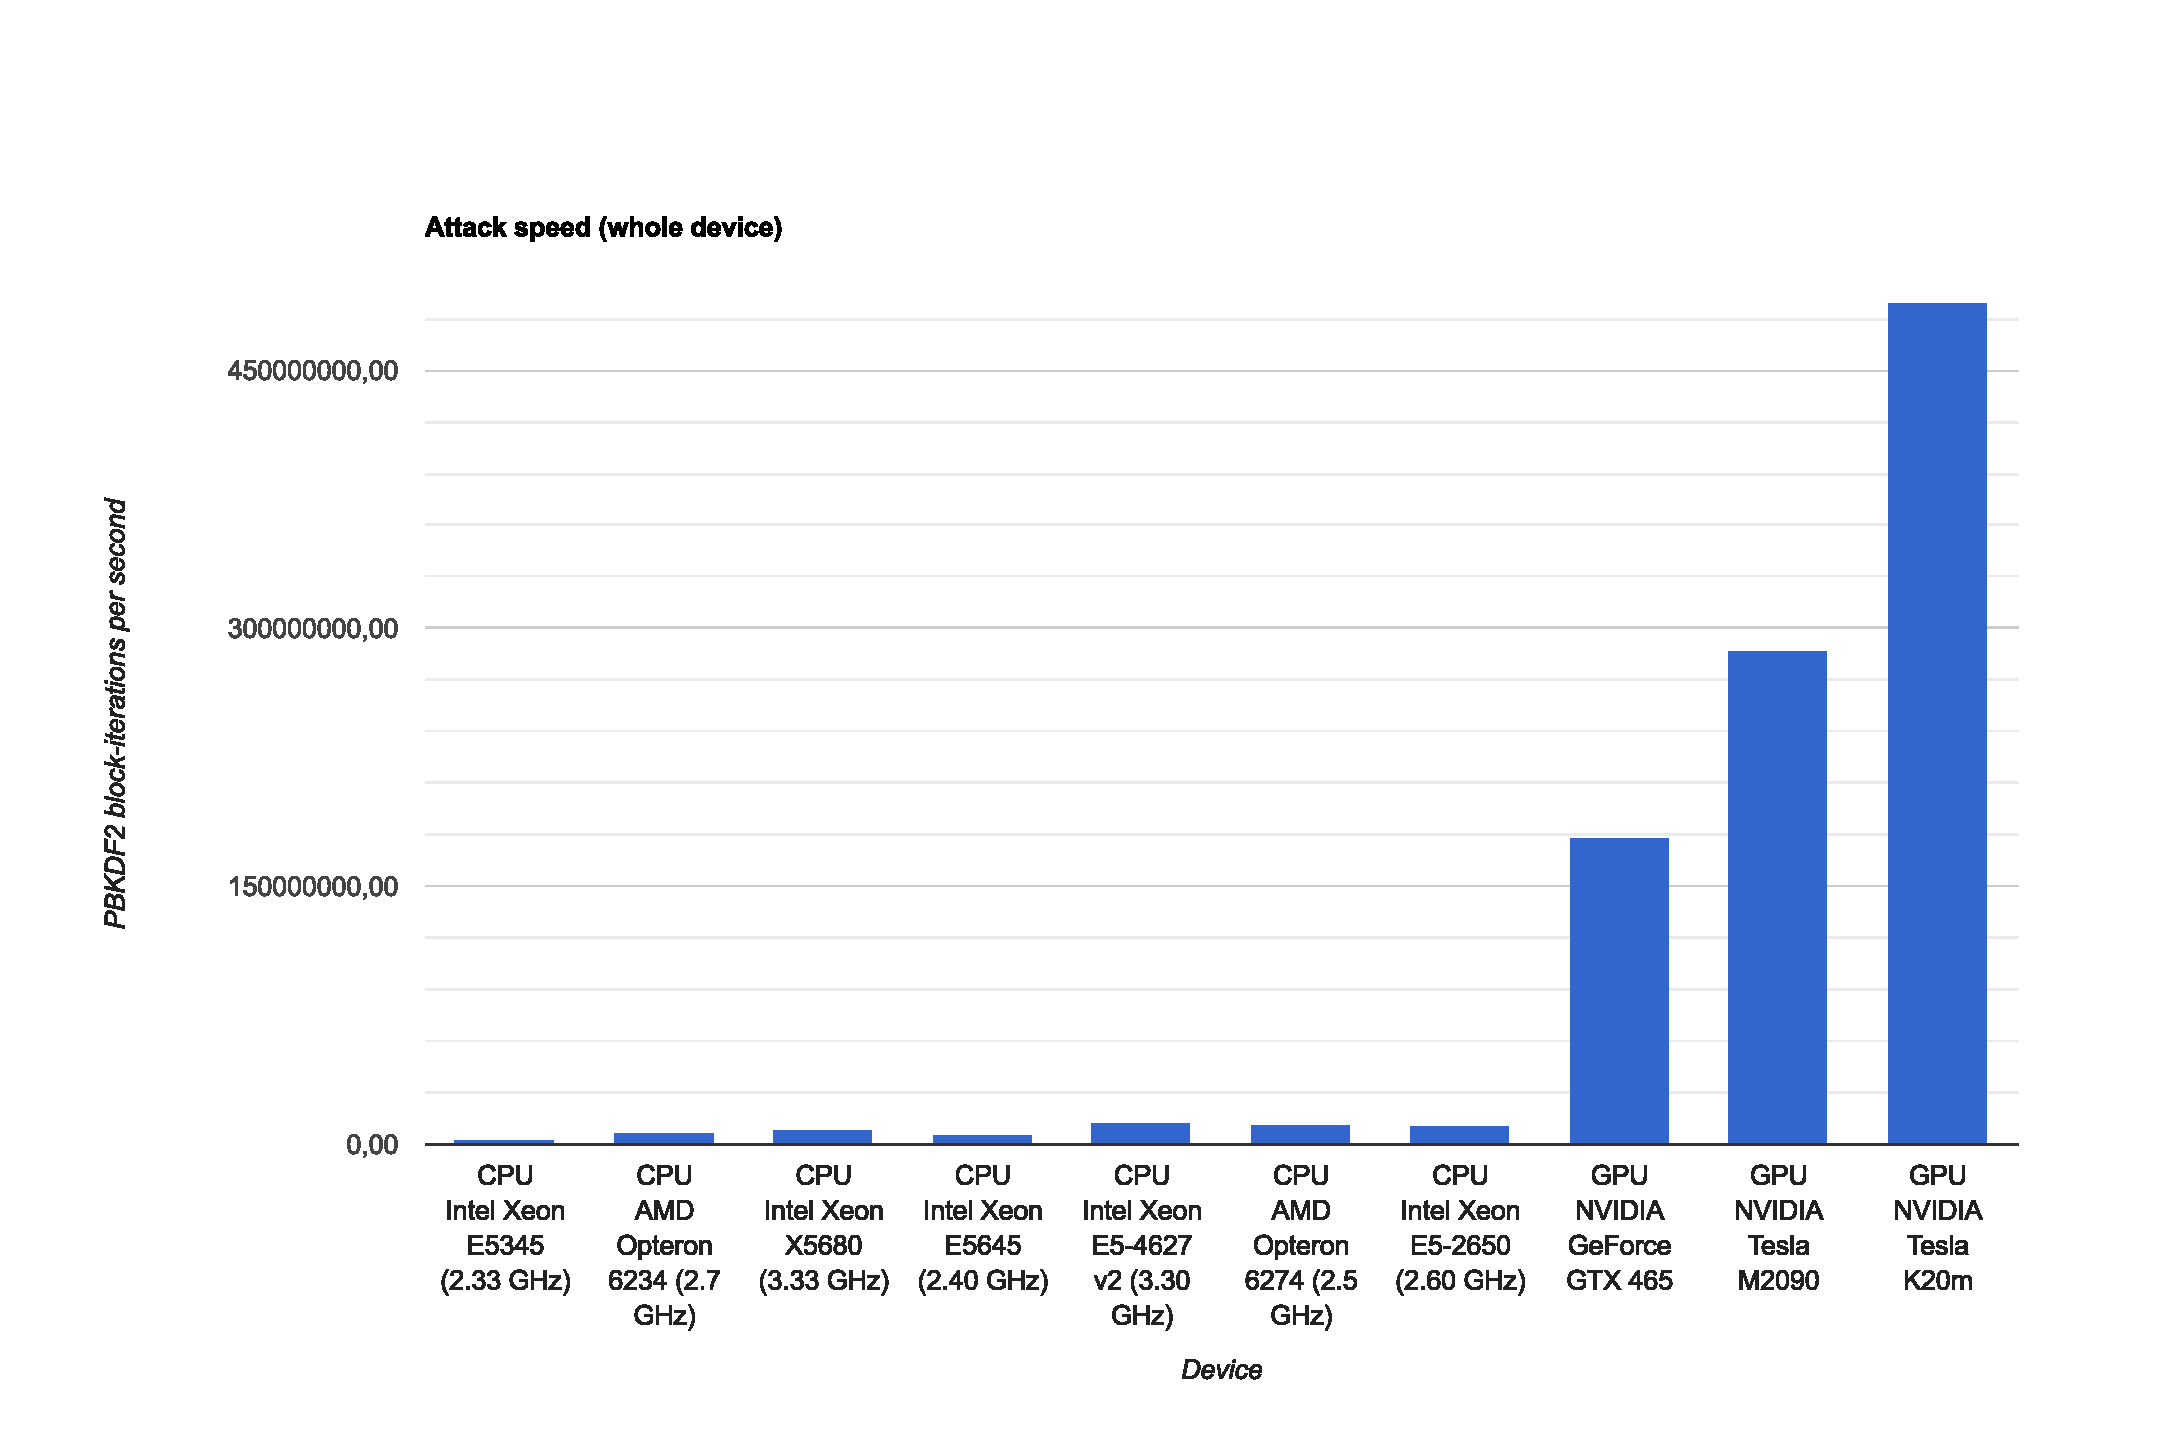
\includegraphics[width=\linewidth, clip=true, trim=1.5cm 0cm 2cm 3cm]{images/devices-raw-speed-whole.eps}
        \caption{PBKDF2-HMAC-SHA1 attack speed per single device}
        \label{graph:devices:speed}
      \end{figure}
      
      The default parameters used in the benchmark were:
      
      ~
      
      \begin{tabular}{l||l|l}
        & \textbf{CPU} & \textbf{GPU} \\
        \hline\hline
        \textbf{Iteration count:} & 4096 & 16384 \\
        \textbf{Derived key length (blocks):} & 16 bytes (1) & 16 bytes (1) \\
        \textbf{Salt length:} & 32 bytes & 32 bytes
      \end{tabular}
      
      ~
      
      Lower iteration count was used for CPU benchmarks only so that they finish within a reasonable time. By measuring the attack speed at different iteration counts we determined that except for extremely low values the iteration count does not influence the attack speed.
      
      The highest attack speed we measured on a CPU was 12.276 million PBIBS (on \emph{Intel Xeon E5-4627 v2}), while the highest attack speed on a GPU was 489.437 million PBIPS (on \emph{NVIDIA Tesla K20m}), which means the attack on a GPU was almost 40 times faster than on a (single) CPU.
      
      For an attacker, however, an increase in attack speed per device alone is probably not going to make a significant difference. Disregarding the initial cost\footnote{An attacker can avoid the initial costs by buying computing power by the hour via a service such as Amazon EC2 (\url{https://aws.amazon.com/ec2/}).}, the the total cost of the attack can be expressed as the product of the attack speed (in work items per second), power consumption at full speed and the price of electricity divided by the number of work items to compute. Therefore, a more meaningful metric would be the attack speed (on a given device) divided by power consumption (of the device while performing the attack).
      
      \begin{figure}
        \centering
        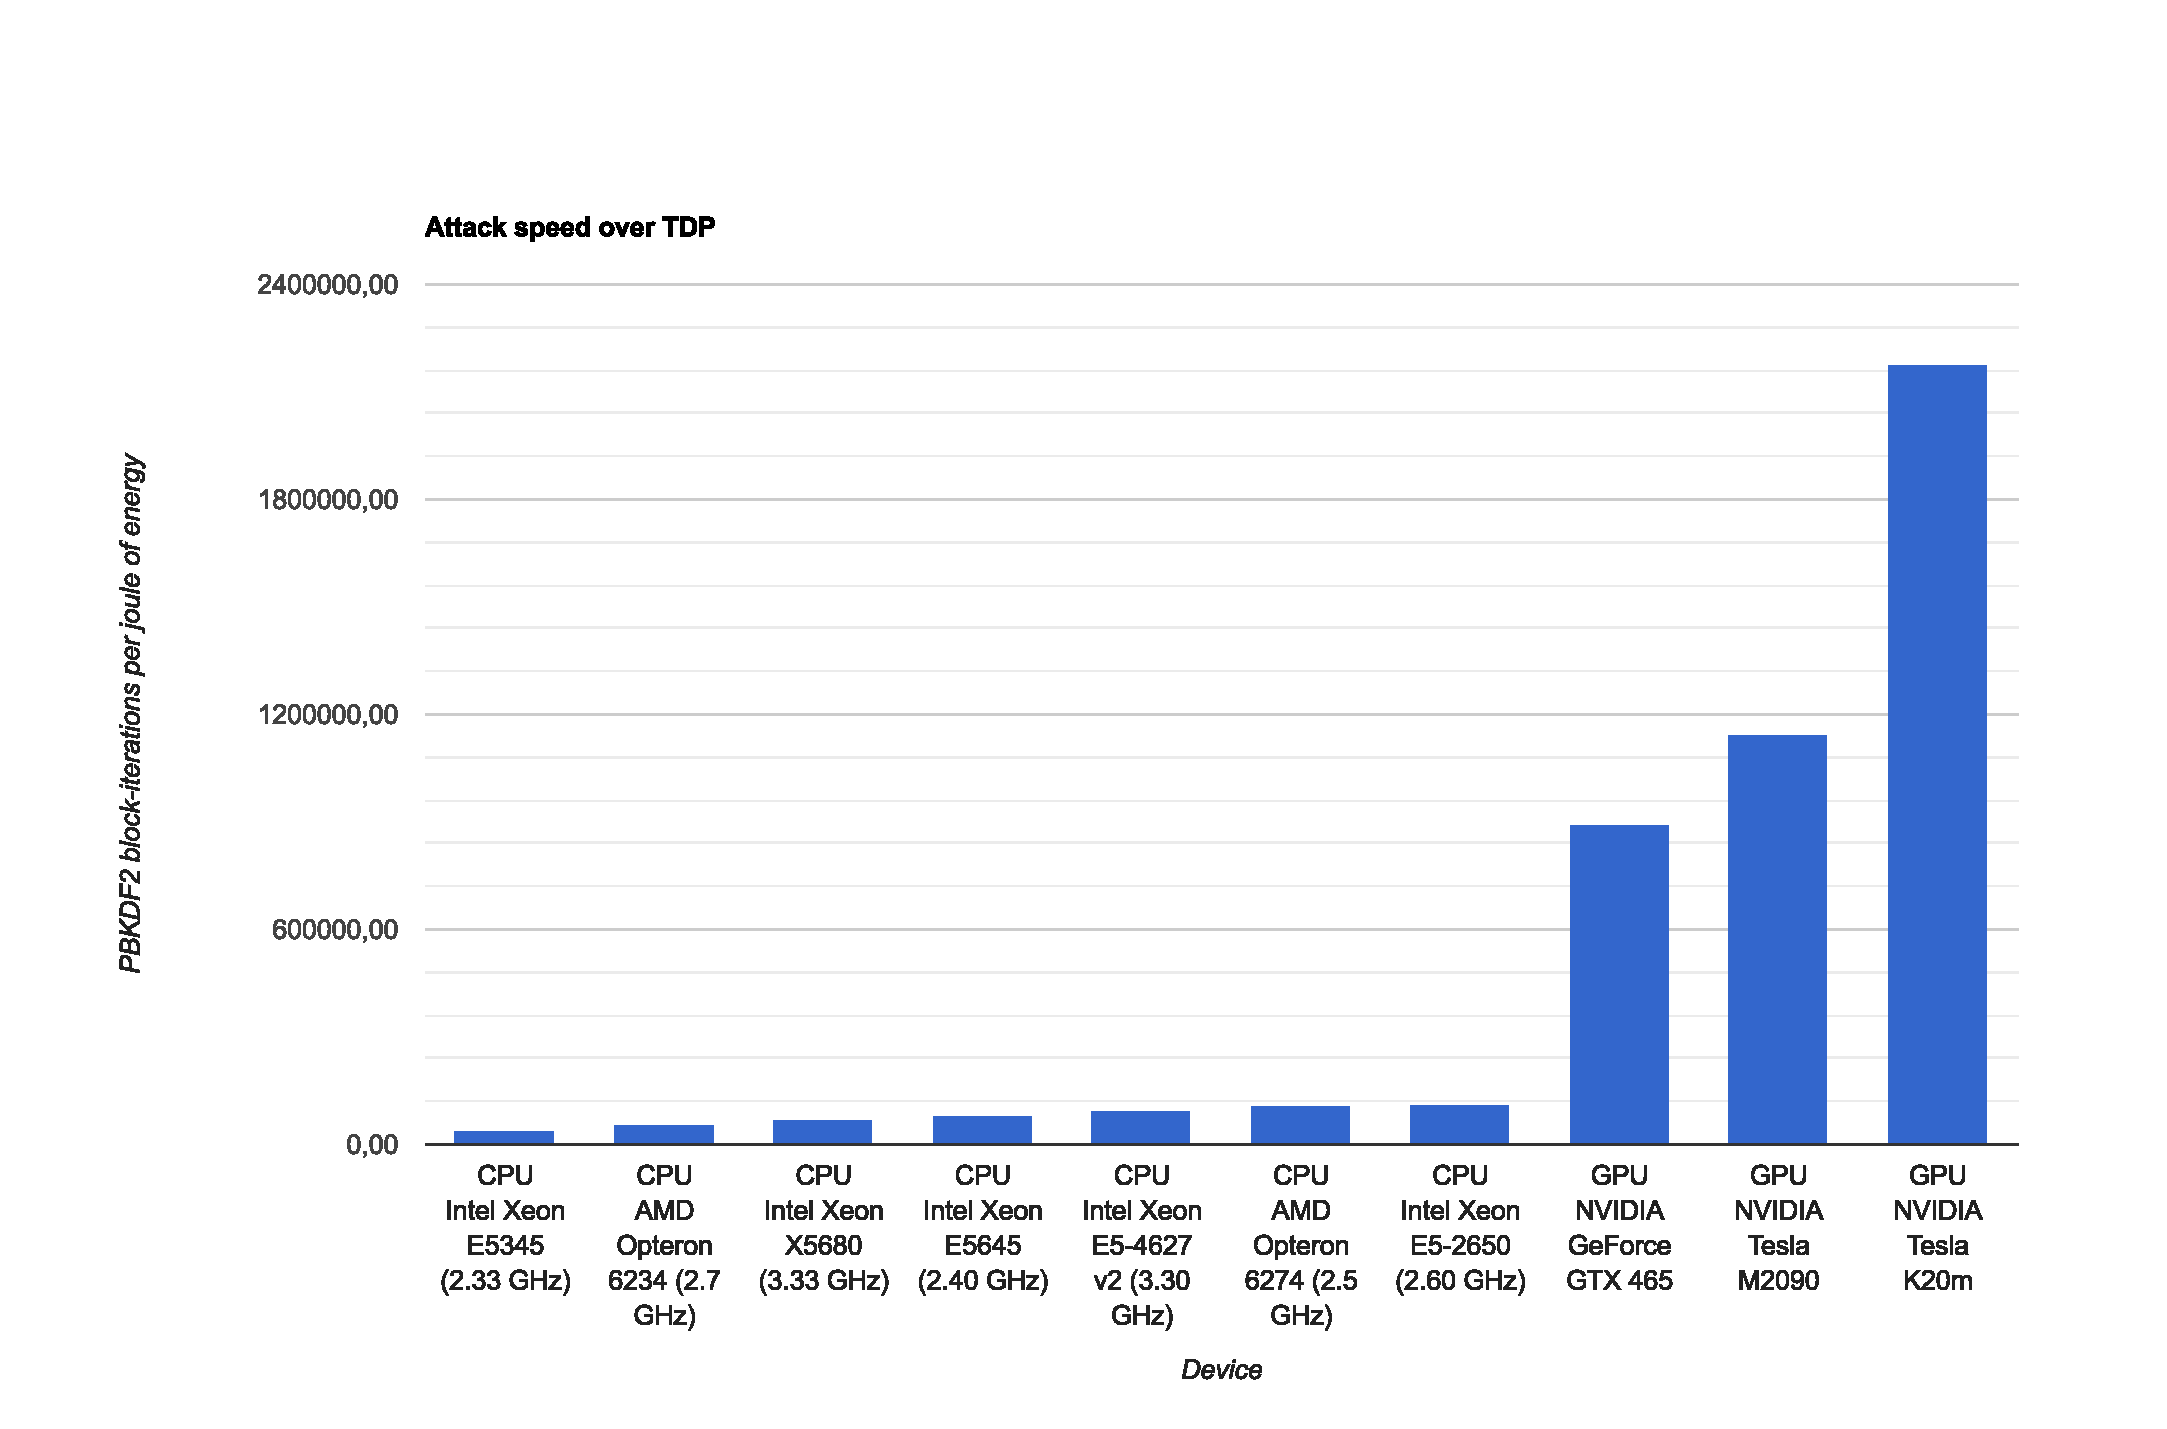
\includegraphics[width=\linewidth, clip=true, trim=1.5cm 0cm 2cm 3cm]{images/devices-power-consumption.eps}
        \caption{PBKDF2-HMAC-SHA1 attack speed over TDP}
        \label{graph:devices:power}
      \end{figure}
      
      In figure \ref{graph:devices:power} the devices are compared by attack speed divided by their thermal design power (TDP). The TDP of a device is defined as the maximum amount of heat generated by the device in typical operation \cite{tdp}. TDP is generally used when designing CPU/GPU cooling systems. However, since almost all of the power drawn by a CPU/GPU eventually converts to heat, it is an acceptable approximation of the actual power consumption.
      
      The highest attack power efficiency we measured on a CPU was 112.385 thousand PBIPJ\footnote{PBIPJ = PBKDF2 block-iterations per joule -- equivalent to PBIPS per watt} (on \emph{Intel Xeon E5-2650}) and the highest attack power efficiency on a GPU was 2\,175.276 PBIPJ (on \emph{NVIDIA Tesla K20m}). This means that the power efficiency of PBKDF2-HMAC-SHA1 processing on a GPU was about 19 times higher than on a CPU.
      
      It should be noted that a GPU cannot operate without at least one CPU, and therefore the actual gain from using a GPU for an attack on PBKDF2 might be lower.
      
    \chapter{Conclusion}
      We analyzed the practicability of an effective brute-force or dictionary attack against PBKDF2 (specifically the most common PBKDF2-HMAC variants with focus on PBKDF2-HMAC-SHA1) performed on GPUs. We have shown that the computation of PBKDF2-HMAC-SHA1 (which is used by default in the disk encryption software \emph{cryptsetup}\footnote{\url{https://gitlab.com/cryptsetup/cryptsetup/wikis/home}} for LUKS encrypted partitions) can be performed significantly faster and more efficiently on a GPU than on a CPU.
      
      We measured a 40-fold difference in speed between the best performing CPU and GPU that we tested. We also found the GPUs to outperform CPUs in terms of power efficiency of the attack. We estimate (based on thermal design power) that the most power efficient GPU (of those that we tested) can perform approximately 20 times more computation than the most power efficient CPU for the same amount of energy consumed. We refer to section \ref{s:results} for more details about the results of our performance benchmarks.
      
      \section{Consequences for applications using PBKDF2}
      Some applications (e. g. Wi-Fi Protected Access protocols in PSK mode \cite{rfc4764} or TrueCrypt \cite{truecrypt}) use only fixed iteration count for PBKDF2 (usually close to the minimum of 1000 iterations recommended in RFC 2898 \cite[section 4.2]{rfc2898}). These applications are particularly vulnerable against GPU attacks, and since they do not update the iteration count based on the steadily increasing hardware performance, they are likely to become even more insecure in the near future.
      
      Other applications (e. g. the LUKS implementation in cryptsetup) try to adapt the iteration count to the current hardware performance by selecting the iteration count based on the time it takes to perform the PBKDF2 computation (usually on the user's hardware). In cryptsetup, when the user sets up an access password for a LUKS encrypted partition, they specify the requested time the computation should take and the iteration count is selected based on this requirement. Although this solution still does not address the problem of upgrading the iteration count regularly after the key setup (the user must do this explicitly) and does not account for potentially more advanced hardware that might be available to the attacker (including GPU hardware), it is a significant improvement as opposed to a fixed iteration count.
      
      To better protect against GPU attacks on passwords, future applications should consider alternative password-based key derivation functions based on sequential memory-hard functions (see sections \ref{s:PBKDFs} and \ref{s:scrypt}). Although these functions have certain drawbacks and are not yet widely adopted, there are active efforts within the cryptographic community to improve this situation, such as the Password Hashing Competition \cite{phc}.
      
      Regardless of these concerns, the best way to protect passwords against brute-force and dictionary attacks remains the choice of long, unpredictable passwords (preferably passphrases).
      
      \section{Future work}
      The PBKDF2 performance benchmarks and comparisons in this work are limited to the PBKDF2-HMAC-SHA1 key derivation function. Since other common hash functions (especially the hash functions from the SHA-2 and SHA-3 families) have higher memory requirements (see section \ref{s:PBKDF2onGPU}), and thus could have less efficient GPU implementations, an evaluation of other key derivation functions from the PBKDF2-HMAC family could prove to be interesting. The software developed as part of this work has been designed to allow extending it with other PBKDF2-HMAC implementations.
      
      Furthermore, the password-based key derivation functions selected as finalists of the Password Hashing Competition \cite{phc} also present as a compelling target for GPU performance evaluation.
      
    \appendix
    \chapter{Software documentation} \label{a:docs}
      This appendix contains the documentation of the software included with this thesis. The source code can be found in the archive file included in the thesis repository. It is also accessible online at \url{https://github.com/WOnder93/pbkdf2-gpu}. The software is written in the C++ language (the C++11 version, standardized in ISO/IEC 14882:2011).
      
      \section{Building the software} \label{s:building}
      The software can be built on most Unix platforms using the GNU build system\footnote{\url{https://www.gnu.org/software/automake/manual/html_node/Autotools-Introduction.html}}. The source code also includes build files for qmake\footnote{\url{http://doc.qt.io/qt-5/qmake-manual.html}}. Building on non-Unix platforms with QMake should be possible, however it hasn't been tested.
      
      The software requires the following libraries to be installed on the target system:
      \begin{itemize}
        \item the OpenSSL\footnote{\url{https://www.openssl.org/}} or LibreSSL\footnote{\url{http://www.libressl.org/}} \emph{crypto} library,
        \item an OpenCL\footnote{\url{https://www.khronos.org/opencl/}} implementation (the OpenCL library implementation is provided by the GPU/CPU manufacturers).
      \end{itemize}
      
      To build the software using the GNU build system, run the following commands in the directory containing the software (the software directory):
      
      \begin{verbatim}
$ autoreconf -i
$ mkdir build && cd build
$ ../configure --disable-shared && make
      \end{verbatim}
      
      \section{Directories}
      The software directory contains the following subdirectories:
      \begin{itemize}
        \item Project directories (source code):
        \begin{itemize}
          \item \verb|libhashspec-openssl| -- a utility library to lookup an OpenSSL hash algorithm (a pointer to the \verb|EVP_MD| structure) from a LUKS \emph{hash-spec} string (see section \ref{s:luks}).
          \item \verb|libhashspec-hashalgoritm| -- a utility library to lookup a hash algorithm implementation based on a LUKS \emph{hash-spec} string.
          \item \verb|libcipherspec-cipheralgorithm| -- a utility library to lookup a cipher algorithm implementation based on LUKS \emph{cipher-spec} and \emph{cipher-mode} string.
          \item \verb|libivmode| -- a utility library to lookup an IV generator implementation based on a LUKS \emph{cipher-mode} string.
          \item \verb|libpbkdf2-compute-cpu| -- a reference implementation of the \emph{libpbkdf2-compute} interface performing computation on the CPU.
          \item \verb|libpbkdf2-compute-opencl| -- an implementation of the \emph{libpbkdf2-compute} interface performing computation on one or more OpenCL devices.
          \item \verb|libcommandline| -- a simple command-line argument parser.
          \item \verb|pbkdf2-compute-tests| -- a utility command-line application that checks the \verb|libpbkdf2-compute-*| libraries against standard test vectors.
          \item \verb|benchmarking-tool| -- a command-line tool for benchmarking the performance of the \verb|libpbkdf2-compute-*| libraries.
          \item \verb|lukscrack-gpu| -- a command-line tool for cracking passwords of LUKS encrypted partitions (the demonstration program).
        \end{itemize}
        
        \item Other directories:
        \begin{itemize}
          \item \verb|data| -- contains the raw data from the benchmarks.
          \item \verb|scripts| -- contains scripts for running the benchmarks.
          \item \verb|examples| -- contains example partition headers and password lists for \emph{lukscrack-gpu}.
          \item \verb|m4| -- contains macros for GNU autoconf.
        \end{itemize}
      \end{itemize}
      
      The \verb|libpbkdf2-compute-*| libraries conform to a common interface which allows writing generic code using C++ templates, which can be used for both CPU and GPU computation. 
      
      \section{Command-line interface}
      This section documents the command-line argument syntax for executable programs and scripts included in the software.
      
      The \emph{benchmarking-tool} and \emph{lukscrack-gpu} programs need to know the path to the data directory containing the OpenCL kernel sources (these are compiled at run time). The directory is located under the software directory in \verb|libpbkdf2-compute-opencl/data|. The OpenCL data directory has to be specified in the command-line when running the programs. By default, these programs expect the directory to be at \verb|./data| (relative to their current directory). When the source code is built using the GNU build system, an appropriate symbolic link with name \verb|data| is created in the containing directory of each program.
      
      The \emph{benchmarking-tool} and \emph{lukscrack-gpu} programs accept a command-line option called \emph{batch size} (\verb|-b, --batch-size|). When running \emph{benchmarking-tool} in CPU mode this option only specifies how many sequential computations of PBKDF2 should be performed (measuring more tasks together in a batch might yield better precision). When running \emph{benchmarking-tool} (in OpenCL mode on a GPU) or \emph{lukscrack-gpu}, batch size specifies the number of PBKDF2 tasks that are submitted to the GPU at once. Therefore it is necessary to set the batch size to a sufficiently large power of two in order to utilize all cores of a GPU. The minimum optimal batch size should be determined for each GPU device and derived key length by a separate benchmark. For example, with NVIDIA Tesla K20m and one derived key block per task the minimum optimal batch size is 65\,536.
      
      \subsection{Benchmarking-tool}
      The \emph{benchmarking-tool} program runs a benchmark several times on a given device and prints the results in a specified format on the standard output stream.
      
      The program accepts the following command-line options:
      \begin{itemize}
        \item \verb|-l, --list-devices| -- When this option is given, the program lists all available devices and exits.
        \item \verb|-m, --mode=MODE| -- Specifies the mode in which to run. When mode \verb|cpu| is set, \emph{libpbkdf2-compute-cpu} is used for PBKDF2 computation; when mode \verb|opencl| is set, \emph{libpbkdf2-compute-opencl} is used for PBKDF2 computation. Default value is \verb|opencl|.
        \item \verb|-d, --device=INDEX| -- Specifies which device to use. The program uses the device at index \emph{INDEX} from the list of devices as reported by \verb|--list-devices|. Default value is \verb|0|.
        \item \verb|-h, --hash-spec=SPEC| -- Specifies the hash function to use. The only supported value is \verb|sha1| (PBKDF2-HMAC-SHA1). Default value is \verb|sha1|.
        \item \verb|-s, --samples=N| -- Specifies the number of times to run the benchmark (the number of samples). Default value is \verb|10|.
        \item \verb|-o, --output-type=TYPE| -- Specifies the type of values to output. Valid values are:
        \begin{itemize}
          \item \verb|iters-per-sec| -- PBKDF2 iterations per second.
          \item \verb|ns| -- the total computation time in nanoseconds.
          \item \verb|ns-per-1M-iters| -- the computations time in nanoseconds per single iteration.
        \end{itemize}
        Default value is \verb|iters-per-sec|.
        \item \verb|    --output-mode=MODE| -- Specifies the mode of output. Valid values are:
        \begin{itemize}
          \item \verb|verbose| -- prints human-readable output.
          \item \verb|raw| -- prints the result for each sample on a separate line.
          \item \verb|mean| -- prints the mean value of all samples.
          \item \verb|mean-and-mdev| -- prints the mean value and mean deviation, each on separate line.
        \end{itemize}
        Default value is \verb|verbose|.
        \item \verb|-i, --iterations=N| -- Specifies the number of iterations for PBKDF2. Default value is \verb|4096|.
        \item \verb|-d, --dk-length=BYTES| -- Specifies the length of derived key in bytes. Default value is \verb|20|.
        \item \verb|    --salt=SALT| -- Specifies the salt to use.
        \item \verb|-b, --batch-size=N| -- Specifies the number of PBKDF2 tasks to submit to the underlying implementation.
        \item \verb|    --opencl-data-dir=DIR| -- Specifies the location of the data directory for the \verb|opencl| mode. Default value is \verb|data|.
        \item \verb|-?, --help| -- When this option is given, the program shows a help text and exits.
      \end{itemize}
      
      \subsection{Lukscrack-gpu}
      The \emph{lukscrack-gpu} program performs a dictionary attack on the access password of a LUKS partition using the specified OpenCL devices.
      
      The program is supplied with a LUKS partition header (which does not have to contain the payload) and a list of passwords to try. The program then performs the attack as described in section \ref{s:demoProgImpl}. If the program finds a valid password, it is printed to the standard output stream terminated by a newline character, otherwise nothing is printed.
      
      \emph{Lukscrack-gpu} only supports the \verb|sha1| hash algorithm for the \emph{hash-spec} field in the LUKS partition header. The cipher algorithms supported are: \verb|aes-ecb| and \verb|aes-cbc| (for keys of 16, 24 and 32 bytes), \verb|aes-xts| (for keys of 32, 48 and 64 bytes), \verb|cast5-ecb| and \verb|cast5-cbc| (for keys of 16 bytes). The initial vector (IV) generators supported are: \verb|plain|, \verb|plain64|, \verb|essiv:sha1|, \verb|essiv:sha256|, \verb|essiv:sha512| and \verb|essiv:ripemd160|.
      
      The program accepts the following command-line options:
      \begin{itemize}
        \item \verb|-l, --list-devices| -- When this option is given, the program lists all available devices and exits.
        \item \verb|-p, --pwgen=list:PWLISTFILE| -- Specifies the password generator to use. The only supported generator is \verb|list:PWLISTFILE| which supplies passwords from file \verb|PWLISTFILE| (\verb|-| is an alias for standard input stream). Default value is \verb|list:-|.
        \item \verb|-k, --keyslot=N| -- Specifies which key slot to attack (0 -- attack first active slot; 1-8 -- attack specific slot).
        \item \verb|-d, --device=INDEX| -- Specifies which devices to use. The program uses the device at index \emph{INDEX} from the list of devices as reported by \verb|--list-devices|. This argument can be given multiple times -- the program then uses all the devices specified. Default value is \verb|0|.
        \item \verb|-t, --threads=N| -- Specifies how many CPU threads to use for CPU computation (see section \ref{s:demoProgImpl} for more details).
        \item \verb|-b, --batch-size=N| -- Specifies the number of PBKDF2 tasks to submit to the underlying implementation.
        \item \verb|-n, --no-newline| -- When this option is present, the program does not print newline after the found password.
        \item \verb|    --opencl-data-dir=DIR| -- Specifies the location of the data directory for the \verb|opencl| mode. Default value is \verb|data|.
        \item \verb|-?, --help| -- When this option is given, the program shows a help text and exits.
      \end{itemize}
      The program accepts a single positional argument -- the path to the file (or block device) containing the LUKS partition header. The partition header file should contain at least the beginning of the raw data from the partition (so that it includes the header and the key material section for the key slot that will be attacked).
      
      \subsection{Scripts}
      The \verb|scripts| directory contains the following executable shell scripts for running benchmarks:
      \begin{itemize}
        \item \verb|run-benchmark.sh| -- a convenience script for running benchmarks.
        \item \verb|run-benchmarks-cpu.sh| -- a convenience script that runs a predefined set of CPU benchmarks.
        \item \verb|run-benchmarks-gpu.sh| -- a convenience script that runs a predefined set of GPU benchmarks.
        \item \verb|run-benchmarks-all.sh| -- runs the above two scripts.
      \end{itemize}
      
      The \verb|scripts/metacentrum| directory contains internal scripts used for performing the benchmarks in the MetaCentrum environment.
      
      The \verb|run-benchmark.sh| script runs a given type of benchmark and stores the results in a comma-separated values (CSV) file. It also stores basic information about the system for future reference in a separate file. It accepts the following positional command-line arguments:
      \begin{enumerate}
        \item the path to the destination directory for the benchmark output files,
        \item the type of benchmark to run (valid values are \verb|simple|, \verb|dl-iter-bs|, \verb|dl-bs|, \verb|salt-len|, \verb|iterations|, \verb|dk-length| and \verb|batch-size|),
        \item the benchmark mode (\verb|cpu| or \verb|gpu|),
        \item an identifier of the benchmark (will appear in the names of the output files),
        \item the directory containing the built binaries (this would be \verb|../biuld| if the software was built using the GNU build system according to section \ref{s:building}),
        \item an optional argument containing the list of environment variables to pass to \emph{benchmarking-tool} (in the syntax of the Unix \verb|env| program).
      \end{enumerate}
      
      The \verb|run-benchmarks-*.sh| scripts must be run their containing directory. They accept four positional arguments which are forwarded to \verb|run-benchmark.sh| as arguments at positions 5, 1, 4, 6 (in this order).
      
      %\section{Running the examples for lukscrack-gpu}
      
    % Bibliography goes here
    % shut up those bibliography warnings:
    \apptocmd{\sloppy}{\hbadness 10000}{}{}
    
    \bibliographystyle{acm}
    \bibliography{thesis}
    
    % Index goes here (optional)
\end{document}
